\documentclass[10pt]{article}
\usepackage{tmlr}

\usepackage{amsmath}
\usepackage{amssymb}
\usepackage{booktabs}
\usepackage{array}
\usepackage{float}
\usepackage{graphicx}
\usepackage{hyperref}
\hypersetup{colorlinks=true,linkcolor=[rgb]{0.10,0.20,0.50},citecolor=[rgb]{0.10,0.35,0.20},urlcolor=[rgb]{0.35,0.10,0.45}}
\usepackage{tikz}
\usetikzlibrary{positioning,arrows.meta}
\usepackage{placeins}
\usepackage{url}

\input{generated/numbers}
\input{generated/tmlr_numbers}
\newcommand{\VfourSymStd}{$+0.357$ $[+0.249,\,+0.464]$}
\newcommand{\VfourAsymStd}{$-0.074$ $[-0.150,\,+0.000]$}
\newcommand{\VfourAsymBoth}{$+0.237$ $[+0.136,\,+0.346]$}
\newcommand{\VfourSymBoth}{$-0.049$ $[-0.117,\,+0.017]$}
\newcommand{\VfourLossBoth}{$+0.188$ $[+0.082,\,+0.266]$}
\newcommand{\VfourAsymNorm}{$+0.237$ $[+0.169,\,+0.305]$}
\newcommand{\VfourAsymSep}{$+0.174$ $[+0.083,\,+0.255]$}
\newcommand{\VfourSymSep}{$+0.160$ $[+0.078,\,+0.254]$}
\newcommand{\VfourSymNorm}{$+0.050$ $[-0.035,\,+0.144]$}
\newcommand{\VfourSymEps}{$+0.258$ $[+0.187,\,+0.330]$}
\newcommand{\VfourSymEpsChange}{$-0.099$ $[-0.243,\,+0.033]$}
\newcommand{\VfourLBFAsymGlobal}{$+0.447$ $[+0.312,\,+0.559]$}
\newcommand{\VfourLBFAsymSep}{$+0.490$ $[+0.315,\,+0.619]$}
\newcommand{\VfourHorizonEnd}{$+0.121$ $[+0.064,\,+0.177]$}
\newcommand{\VfourHorizonStart}{$+0.291$ $[+0.233,\,+0.341]$}
\newcommand{\VfourBaselineStd}{$0.538$}
\newcommand{\VfourBaselineRange}{$0.31$--$0.45$}
\newcommand{\VfourAppliedActorB}{0.0015}
\newcommand{\VfourAppliedActorS}{0.0002}
\newcommand{\VfourCriticNormB}{1,327}
\newcommand{\VfourCriticNormS}{11,965}
\newcommand{\VfourLBFActorShare}{0.83--0.98}
\newcommand{\VfourAgreeControl}{221/240 (92.1\%)}
\newcommand{\VfourBitControl}{164/240}
\newcommand{\VfourAgreeHorizon}{3,289/3,600 (91.4\%)}
\newcommand{\VfourTrajectories}{4,540}
\newcommand{\VfourCoreHours}{1,489}
\newcommand{\VfourEVSepRawB}{0.68}
\newcommand{\VfourEVSepRawS}{0.30}
\newcommand{\VfourEVNormB}{0.67}
\newcommand{\VfourEVNormS}{0.66}
\newcommand{\VfourLBFLossOnly}{$+0.617$ $[+0.394,\,+0.767]$}
\newcommand{\VfourLBFLossOnlyGlobal}{$+0.543$ $[+0.404,\,+0.638]$}
\newcommand{\VfourIsoMaxSupply}{0.055}
\newcommand{\VfiveAsymStart}{$+0.234$ $[+0.165,\,+0.322]$}
\newcommand{\VfiveAsymEnd}{$+0.154$ $[+0.053,\,+0.256]$}
\newcommand{\VfiveSymEnd}{$-0.049$ $[-0.240,\,+0.099]$}
\newcommand{\VfiveSymStart}{$-0.056$ $[-0.147,\,+0.043]$}
\newcommand{\VsixSymGroup}{$+0.150$ $[+0.095,\,+0.226]$}
\newcommand{\VsixAsymGroup}{$+0.168$ $[+0.077,\,+0.240]$}
\newcommand{\VsixSymGroupChange}{$-0.207$ $[-0.336,\,-0.085]$}
\newcommand{\VsixUpdGlobal}{0.39}
\newcommand{\VsixUpdGroup}{0.95}
\newcommand{\VsixUpdNone}{0.96}
\newcommand{\VsixGradGlobal}{0.12}
\newcommand{\VsixRepro}{480/480}
\newcommand{\VsevenSymPlain}{$+0.160$ $[+0.078,\,+0.254]$}
\newcommand{\VsevenAsymPlain}{$+0.174$ $[+0.083,\,+0.255]$}
\newcommand{\VsevenAMPlain}{$+0.050$ $[+0.000,\,+0.100]$}
\newcommand{\VsevenMBPlain}{$+0.285$ $[+0.208,\,+0.363]$}
\newcommand{\VsevenABPlain}{$+0.334$ $[+0.274,\,+0.405]$}
\newcommand{\VsevenSymPop}{$+0.075$ $[-0.032,\,+0.164]$}
\newcommand{\VsevenAsymPop}{$+0.207$ $[+0.141,\,+0.266]$}
\newcommand{\VsevenAMPop}{$+0.268$ $[+0.211,\,+0.317]$}
\newcommand{\VsevenMBPop}{$+0.014$ $[-0.082,\,+0.113]$}
\newcommand{\VsevenABPop}{$+0.282$ $[+0.181,\,+0.380]$}
\newcommand{\VsevenSymChange}{$-0.085$ $[-0.183,\,+0.006]$}
\newcommand{\VsevenAsymChange}{$+0.033$ $[-0.080,\,+0.135]$}
\newcommand{\VsevenAMChange}{$+0.218$ $[+0.143,\,+0.298]$}
\newcommand{\VsevenEVPlainB}{0.68}
\newcommand{\VsevenEVPlainA}{0.49}
\newcommand{\VsevenEVPlainS}{0.30}
\newcommand{\VsevenMeanPlainA}{$-6.6$}
\newcommand{\VsevenSDPlainA}{30.1}
\newcommand{\VsevenMeanPlainM}{$-13.5$}
\newcommand{\VsevenSDPlainM}{32.2}
\newcommand{\VsevenEVPopB}{0.68}
\newcommand{\VsevenEVPopA}{0.64}
\newcommand{\VsevenEVPopS}{0.69}
\newcommand{\VsevenMeanPopA}{$-3.1$}
\newcommand{\VsevenSDPopA}{29.5}
\newcommand{\VsevenMeanPopM}{$-4.8$}
\newcommand{\VsevenSDPopM}{30.4}
\newcommand{\VsevenSigmaRange}{59--426}
\newcommand{\VeightAMonPlain}{$+0.050$ $[+0.020,\,+0.082]$}
\newcommand{\VeightMonBPlain}{$+0.284$ $[+0.234,\,+0.338]$}
\newcommand{\VeightMonMPlain}{$-0.001$ $[-0.051,\,+0.049]$}
\newcommand{\VeightAMonPop}{$+0.246$ $[+0.197,\,+0.300]$}
\newcommand{\VeightMonBPop}{$+0.036$ $[-0.066,\,+0.130]$}
\newcommand{\VeightMonMPop}{$+0.022$ $[-0.046,\,+0.085]$}
\newcommand{\VeightAMonPlainNine}{$[+0.010,\,+0.092]$}
\newcommand{\VeightMatchMeanPlain}{2\%}
\newcommand{\VeightMatchSdPlain}{1\%}
\newcommand{\VeightMonMeanPlain}{$-6.4$}
\newcommand{\VeightMonSdPlain}{29.8}
\newcommand{\VeightMatchMeanPop}{5\%}
\newcommand{\VeightMatchSdPop}{1\%}
\newcommand{\VeightMonMeanPop}{$-3.0$}
\newcommand{\VeightMonSdPop}{29.1}
\newcommand{\VeightBSymPlain}{$+0.162$ $[+0.058,\,+0.262]$}
\newcommand{\VeightBSymPop}{$+0.006$ $[-0.070,\,+0.085]$}
\newcommand{\VeightBChange}{$-0.156$ $[-0.303,\,-0.016]$}
\newcommand{\VeightBChangeNine}{$[-0.344,\,+0.025]$}
\newcommand{\VeightPoolSymPlain}{$+0.159$ $[+0.094,\,+0.231]$}
\newcommand{\VeightPoolSymPop}{$+0.044$ $[-0.021,\,+0.109]$}
\newcommand{\VeightPoolChange}{$-0.115$ $[-0.209,\,-0.032]$}
\newcommand{\VeightPoolChangeNine}{$[-0.239,\,-0.014]$}

\newcommand{\VrevAsymPos}{23/24}
\newcommand{\VrevSymExcl}{3/24}
\newcommand{\VrevSymNeg}{3}
\newcommand{\VrevSymNegSpan}{1.05--1.5M}
\newcommand{\VrevSymPos}{0}
\newcommand{\VrevAsymMin}{+0.099}
\newcommand{\VrevAsymMax}{+0.236}
\newcommand{\VrevCritB}{1,327}
\newcommand{\VrevCritS}{11,965}
\newcommand{\VrevLabelN}{1,280}
\newcommand{\VrevLabelNearS}{1}
\newcommand{\VrevLabelNearP}{619}
\newcommand{\VrevLosoFlips}{none}

\newcommand{\VrvCovRange}{0.88--0.92}
\newcommand{\VrvFalsePos}{0.087--0.096}
\newcommand{\VrvCalLevel}{99\%}
\newcommand{\VrvCalCovMin}{0.94}
\newcommand{\VrvMCShift}{0.007}
\newcommand{\VrvNContrasts}{17}
\newcommand{\VrvHolmKept}{13}
\newcommand{\VrvHolmMaxP}{0.003}
\newcommand{\VrvVerdictsChanged}{0}
\newcommand{\VrvCriticRatio}{0.111}
\newcommand{\VrvActorRatioPre}{0.70}
\newcommand{\VrvPredRatio}{0.078}
\newcommand{\VrvMeasRatio}{0.121}
\newcommand{\VrvPlainAMcal}{$[-0.012,\,+0.112]$}
\newcommand{\VeightClamp}{15}
\newcommand{\VeightNA}{160}

\newcommand{\VdaSkewA}{$-0.12$ (plain) and $-0.27$ (PopArt)}
\newcommand{\VdaSkewM}{$+0.18$ and $-0.02$}
\newcommand{\VdaRetMeanA}{$-104$}
\newcommand{\VdaRetMeanM}{$-185$}
\newcommand{\VdaRetSdA}{113}
\newcommand{\VdaRetSdM}{148}
\newcommand{\VdaETies}{1}
\newcommand{\VdaEMaxDiff}{2\times10^{-16}}


\newcommand{\wcrit}{w_{50}}
\newcommand{\PT}{\mathrm{PT}}
\providecommand{\Description}[1]{}

\title{Shared Gradient Clipping Alters the Effects of Reward Scaling on Finite-Budget Coordination-Collapse Crossings in PPO%
\thanks{Large language models were used as general-purpose assistive tools for editing, code review, and analysis scripting. The authors designed the study, verified the reported results, and take responsibility for the complete submission.}}

\author{Anonymous Authors}

\def\month{MM}
\def\year{YYYY}
\def\openreview{\url{https://openreview.net/forum?id=XXXX}}

\begin{document}
\maketitle

\begin{abstract}
Cooperative multi-agent reinforcement learning can collapse into low-cooperation behavior when local incentives outweigh the team objective. We define an operational estimand for where this happens: the finite-budget crossing $w_{50}$ along a local/team reward-weighting dial at which collapse becomes more likely than not, estimated from behavioral labels with training-seed-block bootstrap intervals. Asking whether a loss-asymmetric reward transform moves it, we find the answer depends on optimizer coupling. In default Stable-Baselines3 PPO on an inventory network, actor and critic share one gradient clip that the critic dominates; scaling both reward branches by seven moves the crossing by \VfourSymStd{} and shrinks the actor's parameter updates to \VsixUpdGlobal{} of baseline. Clipping actor and critic separately restores the updates and removes part of the shift (\VsixSymGroupChange{}); reward normalization removes the detectable remainder, consistent with a critic-target-scale effect we have not isolated. With separate optimizers and normalized rewards, where no symmetric shift is detectable (\VfourSymBoth{}), a loss-only multiplier still moves the crossing relative to the symmetric control (\VfourAsymBoth{}), through \MaxConfirmationBudget{} transitions (\VfiveAsymEnd{}). In Level-Based Foraging an asymmetric transform also moves the crossing, there by penalizing a cooperative action. Crossings stay budget- and configuration-dependent: $w_{50}$ is a comparative instrument, not a critical point.

\end{abstract}

% =======================================================================

\section{Introduction}
\label{sec:intro}

A team of learning agents can fail even when the task has a good cooperative solution: instead of
learning complementary behavior, agents can settle into locally safe, low-cooperation behavior.
We call this \emph{coordination collapse};
in the MARL literature its endpoint is the \emph{lazy-agent}
policy~\citep{liu2023lazy,peng2023curo}, and the underlying private-versus-collective conflict is
the one studied in sequential social dilemmas~\citep{leibo2017multi}. A common design response is to give
each learner part of the team's reward. We study that choice through a local/team \emph{reward-weighting}
dial, $x_i(w)=(1-w)\,r_i^{\mathrm{local}}+w\,r^{\mathrm{global}}$, and summarize where collapse sets in by a
finite-budget behavioral crossing $\wcrit$: the weight at which a fitted collapse probability passes 50\%,
estimated from pre-specified evaluation labels with seed-paired uncertainty.

Reward-transform comparisons along this dial look as if they should be clean. Multiplying every reward by a
positive constant leaves every optimal policy unchanged, and with per-minibatch advantage normalization it
leaves the policy-gradient step of PPO~\citep{schulman2017ppo} approximately unchanged as well. A symmetric
rescaling should therefore not move the crossing, whereas a transform that weights losses more than gains
changes which outcomes the learner prefers and could move it. Practical actor--critic implementations break
this separation. The critic's regression targets are usually not normalized, so their gradient grows with
the reward; and Stable-Baselines3 PPO~\citep{raffin2021sb3} by default clips the norm of the \emph{joint}
actor--critic gradient. When the critic's gradient dominates that joint norm, the clip shrinks
the actor's step in proportion to the reward scale. A change in reward magnitude can then change what is
learned even though it does not change what is optimal.

It is known that PPO's results depend on implementation details~\citep{engstrom2020implementation,andrychowicz2021matters,henderson2018matters},
that value-target scale can be normalized away~\citep{vanhasselt2016popart}, and that cooperative PPO
implementations normalize value targets~\citep{yu2022surprising}. What has not been shown is that one such
detail, a global clip shared by an actor and an unnormalized critic, changes the \emph{conclusion} of a
reward-design comparison in MARL, nor how large that change is on a behavioral threshold measured with paired
uncertainty. We ask three questions.
\textbf{RQ1:} Does a symmetric reward rescaling move the finite-budget crossing under default PPO, and through
which optimizer quantity: pre-clip gradient, applied gradient, or parameter update?
\textbf{RQ2:} Which interventions remove that shift, and what remains when they are applied?
\textbf{RQ3:} With the pathway removed, does a loss-only multiplier still move the crossing relative to
symmetric controls, including one matched to its reward scale?

The contributions, each tied to the evidence that supports it, are:
(i)~\emph{a mechanism for an optimizer confound} (Sections~\ref{sec:mechanism} and~\ref{sec:optimizer};
Table~\ref{tab:hierarchy}). Under default SB3 PPO, symmetric $\times7$ scaling moves the crossing by
\VfourSymStd{}. Per-minibatch logging shows the critic taking the shared clip: the actor's applied gradient
under symmetric scaling is \VsixGradGlobal{} of the baseline's and its parameter update \VsixUpdGlobal{}.
Clipping actor and critic separately restores the update (\VsixUpdGroup{}) and reduces the shift by
\VsixSymGroupChange{}. The remainder, which clipping does not touch, is not detectable under reward
normalization, and in a fresh-seed cohort normalizing only the critic's targets removes it as well
(change \VeightBChange{}), which attributes it to critic target scale at the declared level.
(ii)~\emph{a measurement protocol with checked uncertainty} (Sections~\ref{sec:design} and~\ref{sec:robustness}):
Firth logistic crossings with training-seed-block intervals, pre-registered experiments (\VfourTrajectories{} trajectories,
of which 3,200 address the optimizer mechanism), and a simulation showing that the nominal 95\% intervals
cover at \VrvCovRange{}; every principal verdict is unchanged at a coverage-calibrated \VrvCalLevel{} level.
(iii)~\emph{a conditional asymmetric effect} (Section~\ref{sec:asymmetric}). With the coupling removed and
rewards normalized, a loss-only multiplier raises the crossing relative to the symmetric control
(\VfourAsymBoth{}), through 3.6M transitions. Against a symmetric control whose training-reward mean and
SD track the multiplier arm's under its own policy, the effect remains under both critics, but its size depends
on the critic: with raw value targets it is small (\VeightAMonPlain{}), because a symmetric reward with the same
moments reproduces most of the loss-only shift; with normalized value targets it is large (\VeightAMonPop{}). In Level-Based Foraging an asymmetric transform also moves the
crossing, through a different incentive route (Section~\ref{sec:lbf}).
We use ``boundary'' and ``crossing'' only in this operational, finite-budget sense, not as claims of
phase-like criticality.

Section~\ref{sec:related} positions the work; Section~\ref{sec:method} defines the reward, transforms,
label and estimand; Section~\ref{sec:mechanism} derives the shared-clip pathway;
Section~\ref{sec:design} sets out the experiments and statistics; Sections~\ref{sec:optimizer}
and~\ref{sec:asymmetric} report symmetric and asymmetric transforms; Section~\ref{sec:lbf} turns to a second
environment; Section~\ref{sec:robustness} collects robustness checks; Sections~\ref{sec:limitations}
and~\ref{sec:discussion} state what the results do and do not establish.

% =======================================================================

\section{Related Work}
\label{sec:related}

Cooperative MARL, studied since independent $Q$-learning on shared
tasks~\citep{tan1993multi,busoniu2008comprehensive}, inherits the lazy-agent and
relative-overgeneralization failures in which agents abandon cooperation for a degenerate
policy~\citep{liu2023lazy,peng2023curo,tampuu2017multiagent}. The standard remedy is centralized
credit assignment under CTDE, a centralized critic or factorized value
function~\citep{lowe2017multi,yu2022surprising,sunehag2018vdn,rashid2018qmix,foerster2018counterfactual,son2019qtran};
related work ties the failure to decentralized exploration and parameter sharing, and locates an
empirical collapse threshold over payoff harshness for each exploration level, averaged over 30
seeds~\citep{weng2026}, or shows decentralized shaping cannot match centralized
baselines~\citep{dmarl2025}. This establishes \emph{that} centralization helps, \emph{how} to implement
it, and that collapse thresholds can be measured. It does not provide a 50\% collapse-probability
crossing along a local/team reward-weighting dial with seed-paired intervals, or test how reward
transforms and optimizer implementation move it. Combined
individual-and-team reward design has direct precedent: DE-MADDPG separates a per-agent and a team
critic for such mixtures~\citep{demaddpg2020}, packet-routing work studied the lazy-versus-selfish
trade-off with mixed and adaptive local/global signals~\citep{mao2020reward}, IRAT
learns individual- and team-reward policies with mutual discrepancy constraints~\citep{wang2022irat},
and CLOT balances individual and team optimization through a Lagrangian
multiplier~\citep{zhang2026clot}. These set or adapt the mixture as a design choice rather than
\emph{locating} a crossing with uncertainty.

Statistically, a 50\% crossing is an effective-dose or psychometric-threshold estimand. Dose--response
analysis routinely estimates ED50 values and differences between them~\citep{ritz2015dose}, and
psychometric work studies bootstrap uncertainty and grid placement~\citep{wichmann2001psychometric}.
We import that logic into trained multi-agent populations; our contribution lies in the experimental
unit, collapse label, seed-block resampling, bracketing diagnostics and paired comparison of reward
designs. Treating collective learning as a dynamical system with critical points has precedent in
phase diagrams over environmental axes~\citep{yamaguchi2025}, metastable opinion-dynamics
boundaries~\citep{capannoli2026phase}, and mean-field limits of multi-agent
learning~\citep{hu2019meanfield,barfuss2019deterministic,hussain2025convergence}; ours is a
reward-structure threshold estimated from trained populations rather than asserted to be a dynamical
critical point.


PPO's behavior depends on implementation details that are not part of the algorithm's
definition~\citep{engstrom2020implementation,andrychowicz2021matters,henderson2018matters}, among them reward
or value normalization~\citep{vanhasselt2016popart} and gradient-norm clipping, which was introduced to bound
exploding gradients~\citep{pascanu2013difficulty}; cooperative PPO implementations normalize value targets by
default~\citep{yu2022surprising}. \citet{andrychowicz2021matters} vary, among many choices, whether actor and
critic share a network and how gradients are clipped, and measure returns. We hold the algorithm fixed and ask a
narrower question: whether one combination of these defaults, a global clip shared by actor and critic without
value normalization, changes the answer to a reward-design question, and through which of the gradient,
applied-gradient and parameter-update quantities it does so.

Human preference structure has entered collective learning only narrowly.
\citet{hughes2018inequity} show inequity aversion improves cooperation within the cooperative-AI
agenda~\citep{dafoe2020open,hammond2025multiagent,barfuss2020caring}; KTO aligns language models with a
Kahneman--Tversky value function carrying an explicit loss-aversion
coefficient~\citep{ethayarajh2024kto}; risk-sensitive RL optimizes tail
outcomes~\citep{qiu2021rmix,xie2023riskq,prashanth2014cvar,tamar2015optimizing}; and prospect theory has
entered single-agent RL with known calibration
concerns~\citep{prashanth2016cumulative,rabin2000risk,tversky1992}. \citet{mengesha2025} find loss
aversion non-monotone in an evolutionary quantal-response model, and \citet{lalmohammed2025} bring CPT
into cooperative MARL inside the actor--critic update, varying value and probability-weighting
components jointly with the optimizer. Unlike inequity aversion, which penalizes the \emph{difference}
between own and peer payoffs, our transform acts on the already-blended scalar against a fixed
reference, so it changes the magnitude and sign-weighting of the training signal rather than the
local-versus-collective trade-off itself.

% =======================================================================

\section{Problem Formulation and the Finite-Budget Crossing}
\label{sec:method}

We study \emph{reward-mixed} cooperative MARL, in which each learner's scalar reward is the blend
$x_i(w)=(1-w)\,r_i^{\mathrm{local}}+w\,r^{\mathrm{global}}$, $w\in[0,\allowbreak 1]$. On the supply
chain the team reward sums the five trained nodes' profits, so
$x_i(w)=r_i^{\mathrm{local}}+w\sum_{j\neq i}r_j^{\mathrm{local}}$: node $i$'s own profit keeps unit
weight and $w$ adds teammates' profits. We do not rescale $r_i^{\mathrm{local}}$ or
$r^{\mathrm{global}}$ at each $w$, so a given $w$ means the same mixture in every condition; the scale of
$x_i$ therefore varies with $w$, which matters under the optimizer coupling studied in
Section~\ref{sec:optimizer}. Each experiment varies one factor at a time. The primary substrate is
\texttt{NetworkManagement-v1}~\citep{hubbs2020orgym}, a six-node multi-echelon inventory
network~\citep{oroojlooyjadid2022,gijsbrechts2022,marlim2023} wrapped with
PettingZoo/SuperSuit~\citep{terry2021pettingzoo,terry2020supersuit}; the second environment is
Level-Based Foraging (Section~\ref{sec:lbf}).

The boundary estimate follows four steps: fix the environment, learner, horizon, and collapse
label; train matched policies across a grid of $w$; label each run from pre-specified
\emph{evaluation} behavior, not training reward; and fit a monotone binary model
$P(\mathrm{collapse}\mid w)$, reporting the midpoint $\wcrit$ with bootstrap confidence intervals.

\paragraph{Information structure.}
The supply-chain experiments train one policy, shared by the five trainable nodes, on each node's own
blended reward. Every node's policy input is the \emph{same} full observation of the network state; there is
no agent identifier, and actions are padded to the largest per-node action dimension, each node using its
leading entries. Under deterministic evaluation the five nodes therefore receive the same action vector. The
setting is thus a fully observed, homogeneous shared controller trained on per-node mixed rewards, not a
decentralized partially observed team: collapse here is the shared policy settling on the lazy action, and
nothing below is evidence about decentralized information. In Level-Based Foraging each agent's actor sees
only its own observation and a centralized critic sees the global state (Section~\ref{sec:lbf}).

\paragraph{Reward transforms.}
With zero as the gain/loss reference, $v(x)=x^\alpha$ for $x\ge0$ and $-\lambda(-x)^\beta$ for $x<0$.
The exponents $\alpha,\beta\in(0,\allowbreak 1]$ control \emph{curvature}; the multiplier $\lambda>1$
scales the loss branch. For $a>0$, $|v(-a)|/v(a)=\lambda a^{\beta-\alpha}$, which equals $\lambda$ at
every magnitude only when $\alpha=\beta$, as in all our experiments. The transform is applied after
blending,
\begin{equation}
 r_i^{\PT}=v\!\left((1-w)\,r_i^{\mathrm{local}}+w\,r^{\mathrm{global}}\right).
 \label{eq:reward}
\end{equation}
Controls use $r_i^{\PT}=v((x_i-z_0)/s_{\mathrm{in}})/s_{\mathrm{out}}$ with no addition of $z_0$ after
transformation; Equation~\ref{eq:reward} has $z_0=0$ and $s_{\mathrm{in}}=s_{\mathrm{out}}=1$. The scale
controls of Section~\ref{sec:optimizer} use the frozen empirical-mean reference $z_0=-2.6281398333$
(Appendix~\ref{app:configuration}) with $u=x-z_0$ and $\phi(u)=\mathrm{sign}(u)|u|^{.88}$: arm
B$=\phi(u)$ (curvature only), A$=v_7(u)$ (losses $\times7$), S$=7\phi(u)$ (both branches $\times7$,
i.e.\ $s_{\mathrm{out}}=1/7$), and R$=3.451\,\phi(u)$ (both branches scaled by A's pooled RMS ratio).
We omit the probability-weighting channel of full CPT. Unlike \citet{lalmohammed2025}, the transform
sits outside the optimizer, so within a fixed optimizer configuration matched runs differ only in the
scalar training signal.

\paragraph{Collapse label.}
A \emph{collapse label} is a pre-specified binary evaluation rule scored on held-out evaluation
episodes. In the supply chain, collapse is $\mathbf{1}[\bar S<10\wedge\bar\pi\le-127.1]$, where
$\bar\pi$ is the total profit of nodes 2--6 averaged over ten deterministic evaluation episodes
(seeds $10s,\dots,10s+9$ for training seed $s$) and $\bar S$ is the mean over the five trained nodes of
the deterministic base-stock target $250(a_1+1)$ chosen at the reset of the first evaluation episode,
where $a_1$ is the node's first action component. Node 1 is scripted to order 20 units, split equally
across its action entries. Collapsed runs sit at the lazy-policy profit floor ($\approx-128$), so the
profit clause is a redundancy check on $\bar S<10$; threshold variants of $\pm20\%$ change $\wcrit$ by
at most 0.015. Across all \VrevLabelN{} E1 runs only \VrevLabelNearS{} has $\bar S$ within one unit of the
threshold, so the label is not a fine cut through a continuum (Figure~\ref{fig:label}, Appendix~\ref{app:factorial}).

\paragraph{Estimand.}
We write the estimand as $w_{50}(T;E,A,V,U,L,Q)$: training budget, environment, learner (including its
optimizer configuration), transform, reward units, collapse label and evaluation protocol. It is a
fitted 50\% crossing, not a safe operating point, and a rightward shift means more team weight is needed
to reach it. We fit $P(\mathrm{collapse}\mid w)=\sigma(b_0+b_1w)$ and report $\wcrit=-b_0/b_1$
(Section~\ref{sec:design}). Collapse becomes less likely as $w$ grows, so $b_1<0$ in every fit we report.

% =======================================================================

\section{The Shared-Clip Pathway in PPO}
\label{sec:mechanism}

\paragraph{Learner and optimizer.}
The supply-chain learner is parameter-shared PPO in Stable-Baselines3 2.8.0~\citep{raffin2021sb3}:
one policy across nodes, separate actor and critic MLPs, a single Adam optimizer ($\epsilon=10^{-5}$,
SB3's implicit default) over both, advantages normalized per minibatch, no value normalization, and one
global gradient-norm clip of 0.5 applied to the concatenated actor and critic gradient. Because the
actor's advantages are normalized but the critic's targets are not, a larger reward scale enlarges only
the value-loss gradient, which then dominates the shared clip. Section~\ref{sec:optimizer} varies
exactly this coupling. Training budgets count requested agent transitions; with five trained lanes and
128-step rollouts each rollout adds 640 transitions, so 300k requested transitions execute 300,160
(Appendix~\ref{app:configuration}).

\paragraph{How reward scale reaches the actor.}
Write the PPO loss as $\mathcal L=\mathcal L_\pi(\theta_a)+c_v\,\mathcal L_V(\theta_c)$ with value-loss coefficient
$c_v=0.5$ and no entropy term, where the actor parameters $\theta_a$ and critic parameters $\theta_c$ are
disjoint (the networks share no trainable parameter). On a minibatch let $g_a=\nabla_{\theta_a}\mathcal L$
and $g_c=\nabla_{\theta_c}\mathcal L$. SB3 rescales the concatenated gradient to norm at most $\tau=0.5$,
\begin{equation}
\tilde g=\kappa\,(g_a,g_c),\qquad \kappa=\min\!\Bigl(1,\;\frac{\tau}{\sqrt{\|g_a\|^2+\|g_c\|^2}}\Bigr),
\qquad\text{so}\qquad \|\tilde g_a\|=\kappa\|g_a\|\approx\tau\,\frac{\|g_a\|}{\|g_c\|}\ \ \text{when}\ \|g_c\|\gg\|g_a\|.
\label{eq:clip}
\end{equation}
Multiply every reward by $s>0$. Returns, value targets and, at a fixed relative fit, the value error scale by
$s$, so $\|g_c\|=c_v\|\nabla_{\theta_c}\tfrac12(V-\hat R)^2\|$ scales by about $s$; the advantages also scale by
$s$, but are normalized per minibatch, so $\|g_a\|$ does not. By Equation~\ref{eq:clip} the applied actor
gradient then falls by about $1/s$. Clipping actor and critic \emph{separately} replaces $\kappa$ with
$\kappa_a=\min(1,\tau/\|g_a\|)$, which does not involve the critic, and normalizing rewards or value targets
keeps $\|g_c\|$ from growing with $s$. Adam~\citep{kingma2015adam} divides each coordinate by a running
root-mean-square of its own gradient, so it would undo a \emph{constant} rescaling of $\tilde g_a$. It does not
fully undo this one, because $\kappa$ varies from minibatch to minibatch with the critic's error and because
the denominator is floored at $\epsilon$. The applied gradient is therefore not the quantity that reaches the
policy; the parameter update is, and it is what E6 measures directly. We do not isolate how much of the
remaining attenuation is due to the varying $\kappa$ and how much to $\epsilon$.

The argument makes four testable predictions, which Section~\ref{sec:optimizer} checks in turn:
(a)~under the shared clip the critic's pre-clip norm grows with the reward multiplier while the actor's does
not; (b)~the actor's applied gradient, and to a lesser degree its parameter update, shrink under symmetric
scaling; (c)~per-group clipping restores the actor's update and removes the part of the crossing shift that
runs through $\kappa$; (d)~what remains after (c) runs through the critic's targets, so normalizing rewards
or targets should remove it. As a quantitative check of (b), we evaluated Equation~\ref{eq:clip} on every logged minibatch of the default
cell. The critic accounts for more than 99.99\% of the squared joint norm in both arms, every minibatch is clipped,
and the predicted S/B ratio of applied actor gradients, \VeqPred{}, equals the measured \VeqMeas{} (largest
per-minibatch relative error $\VeqMaxErr{}$); under per-group clipping both are \VeqGroupMeas{}. Because
Equation~\ref{eq:clip} is how the clip is computed, this check does not test the clip itself. What it establishes
is that the clip acts on the joint norm, that $\kappa\approx\tau/\|g_c\|$ throughout, and that the actor's
attenuation is fully accounted for by the critic's gradient. Evaluating the formula at cell-mean norms instead gives
\VrvPredRatio{}, because those norms are heavy-tailed. Figure~\ref{fig:mechanism} summarizes the pathway and
where each intervention acts.

\begin{figure}[!htbp]
\centering
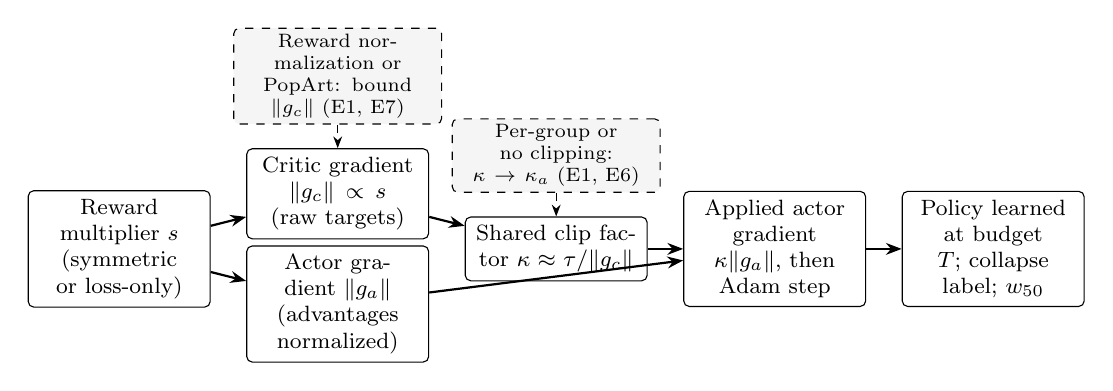
\begin{tikzpicture}[node distance=4mm and 4.5mm, every node/.style={font=\footnotesize, align=center},
  box/.style={draw, rounded corners=2pt, minimum height=8mm, inner sep=3pt, text width=21mm, fill=white},
  inter/.style={draw, dashed, rounded corners=2pt, inner sep=2pt, text width=25mm, fill=black!4, font=\scriptsize},
  arr/.style={-{Stealth[length=2mm]}, thick}]
\node[box] (r) {Reward multiplier $s$ (symmetric or loss-only)};
\node[box, right=of r, yshift=7mm] (c) {Critic gradient $\|g_c\|\propto s$ (raw targets)};
\node[box, right=of r, yshift=-7mm] (a) {Actor gradient $\|g_a\|$ (advantages normalized)};
\node[box, right=of c, yshift=-7mm] (k) {Shared clip factor $\kappa\approx\tau/\|g_c\|$};
\node[box, right=of k] (u) {Applied actor gradient $\kappa\|g_a\|$, then Adam step};
\node[box, right=of u] (b) {Policy learned at budget $T$; collapse label; $w_{50}$};
\draw[arr] (r) -- (c); \draw[arr] (r) -- (a); \draw[arr] (c) -- (k); \draw[arr] (a) -- (u); \draw[arr] (k) -- (u); \draw[arr] (u) -- (b);
\node[inter, above=3mm of c] (i1) {Reward normalization or PopArt: bound $\|g_c\|$ (E1, E7)};
\node[inter, above=3mm of k] (i2) {Per-group or no clipping: $\kappa\to\kappa_a$ (E1, E6)};
\draw[dashed, -{Stealth[length=1.5mm]}] (i1) -- (c); \draw[dashed, -{Stealth[length=1.5mm]}] (i2) -- (k);
\end{tikzpicture}
\caption{The shared-clip pathway. A reward multiplier enlarges the critic's gradient when value targets are not normalized, but not the actor's, because advantages are normalized per minibatch. A global clip shared by both then shrinks the actor's applied gradient roughly in proportion to $1/\|g_c\|$; Adam partly, but not fully, compensates. Dashed boxes mark where the interventions act and which experiments test them. The measured quantities are, from left to right: pre-clip norms (E1, E6), applied actor gradient and parameter update (E6), and crossing contrasts (all experiments).}
\label{fig:mechanism}
\Description{Flow diagram from reward multiplier to critic gradient and actor gradient, through a shared clip factor to the applied actor gradient and Adam step, to the learned policy and crossing; two dashed intervention boxes point at the critic gradient and the clip factor.}
\end{figure}

% =======================================================================

\section{Experimental Design and Statistical Methodology}
\label{sec:design}

\begin{table*}[t]
\caption{Experimental setup. Legacy sweeps (earlier platform, 20 seeds per cell) supply the 300k decomposition and the cross-sectional horizon fit; pre-registered experiments E1--E6 run on one platform with ten seeds per cell.}
\label{tab:setup}
\centering\scriptsize
\begin{tabular}{@{}>{\raggedright\arraybackslash}p{.15\textwidth}>{\raggedright\arraybackslash}p{.395\textwidth}>{\raggedright\arraybackslash}p{.395\textwidth}@{}}
\toprule
 & Supply chain (legacy, E1--E3) & Level-Based Foraging (E4) \\
\midrule
Environment & Six-node \texttt{NetworkManagement-v1}; node 1 scripted, nodes 2--6 trained; 30-period episodes. & \texttt{Foraging-5x5-2p-2f-v3}; two players, two foods; 50-step episodes. \\
Local reward & Node $i$'s period profit (revenue minus procurement, operating, holding, pipeline and unfulfilled-demand costs). & Native food share minus 0.02 per LOAD attempt. \\
Team reward & Sum of the five trained nodes' profits. & Sum of native food rewards. \\
Learner & Parameter-shared PPO (SB3 2.8.0); separate actor and critic MLPs. & MAPPO: actor on own observation, critic on global state (SB3 2.8.0). \\
Optimizer & Default: one Adam step ($\epsilon=10^{-5}$), global clip 0.5, no value normalization. E1 adds separate no-clip optimizers and \texttt{VecNormalize}; E2 sets $\epsilon=10^{-8}$; E6 clips actor and critic separately; E5 uses the fully decoupled learner. & Global clip 0.5 or separate no-clip optimizers. \\
Collapse label & $\mathbf 1[\bar S<10\wedge\bar\pi\le-127.1]$ on ten deterministic evaluation episodes. & Native team return $<0.626$ over ten evaluation episodes (no effort cost). \\
Arms & Linear; curvature $\alpha{=}\beta{=}.88$ with $\lambda\in\{1,\ldots,7\}$ (legacy); B, A ($\lambda=7$), S ($\times7$), R ($\times3.451$) with $z_0=-2.628$ (E1, E2); linear, curvature, $\lambda=7$ (E3); B, A, S (E5, E6). & Linear; curvature; A ($\lambda=4$); S (both branches $\times4$). \\
Budget, grid & 300k, eight cells (E1, E2); 3.6M with 24 checkpoints, nine cells (E3, E5). & 2M timesteps; ten cells $\{0,.1,.2,.3,.5,.65,.75,.85,.9,.95\}$. \\
Uncertainty & \multicolumn{2}{>{\raggedright\arraybackslash}p{.80\textwidth}}{Firth logistic midpoint; 2,000 multinomial draws of complete training-seed blocks, shared across conditions so that contrasts are paired.} \\
\bottomrule
\end{tabular}
\end{table*}


\begin{table}[!htbp]
\caption{Experiment matrix. All experiments use ten training seeds (42--51) per arm and mixture cell, one evaluation label per run, the Firth crossing and seed-block bootstrap intervals (E8's replication cohort uses seeds 52--61); E4 runs on Level-Based Foraging, all others on the supply chain. E1--E4 were pre-registered together, E5--E8 each before any of its runs. ``Main finding'' cites the contrast that answers the row's question; Table~\ref{tab:results} gives intervals.}
\label{tab:matrix}
\centering\scriptsize\setlength{\tabcolsep}{3pt}
\begin{tabular}{@{}>{\raggedright\arraybackslash}p{.045\textwidth}>{\raggedright\arraybackslash}p{.15\textwidth}>{\raggedright\arraybackslash}p{.21\textwidth}>{\raggedright\arraybackslash}p{.17\textwidth}>{\raggedright\arraybackslash}p{.06\textwidth}>{\raggedright\arraybackslash}p{.15\textwidth}>{\raggedright\arraybackslash}p{.12\textwidth}@{}}
\toprule
ID & Question & Design (baseline $\to$ intervention) & Arms, grid, budget & Runs & Main finding & Main limitation \\
\midrule
E1 & RQ1--3: does reward scale or shape move $w_{50}$, by optimizer? & \{shared clip, separate no-clip optimizers\} $\times$ \{raw, normalized rewards\} & B, A, S, R; 8 cells; 300k & 1,280 & Default: S$-$B large; decoupled: S$-$B not detectable, A$-$S positive & A, S differ in reward mean \\
E2 & Is Adam's $\epsilon$ the route? & Default with $\epsilon=10^{-8}$ & B, A, S, R; 8 cells; 300k & 320 & S$-$B unchanged & Update norms not logged \\
E3 & Budget dependence, default learner & Default learner to 3.6M, 24 checkpoints & linear, curvature, $\lambda=7$; 9 cells & 270 & Contrast shrinks; no stable crossing & Includes scale pathway \\
E4 & Second environment & MAPPO on LBF; shared clip vs separate optimizers & linear, curvature, A, S; 10 cells; 2M & 800 & A$-$S positive in both modes & Label fallback (D4); estimator sensitivity \\
E5 & Does A$-$S persist with budget? & Decoupled learner to 3.6M, 24 checkpoints & B, A, S; 9 cells & 270 & A$-$S positive at all primary budgets & Pointwise intervals \\
E6 & Is the shared clip the pathway? & Shared vs per-group vs no clipping; update logging & B, A, S; 8 cells; 300k & 720 & Per-group clip restores update, reduces S$-$B & Residual unexplained \\
E7 & Critic targets? Reward moments? & Plain vs PopArt critic; scale-matched control M & B, A, S, M; 8 cells; 300k & 400 new + 240 E1 & PopArt: inconclusive; A$-$M separable only with PopArt & M's mean unmatched \\
E8 & Moments or shape? Critic targets, fresh seeds? & Online moment-matched control M$_{\mathrm{on}}$; B, S on seeds 52--61 & M$_{\mathrm{on}}$; B, S; 8 cells; 300k & 480 & A$-$M$_{\mathrm{on}}$ small (plain), large (PopArt); PopArt removes S$-$B & Map nonstationary; 99\% level \\
\bottomrule
\end{tabular}
\end{table}

\paragraph{Experiments.}
Table~\ref{tab:matrix} lists the eight pre-registered experiments. Together they comprise \VfourTrajectories{}
trajectories; the 3,200 in E1, E2, E6, E7 and E8 address the optimizer mechanism, E3 and E5 follow 540 trajectories to 3.6M
transitions, and E4's 800 run on the second environment. Earlier ``legacy'' sweeps from another platform
(20 seeds per cell) supply the curvature-versus-multiplier decomposition and the cross-sectional horizon
fit; they are reported separately and never pooled with E1--E8.

\paragraph{Estimation.}
We fit the logistic curve by Firth's bias-reduced maximum likelihood~\citep{firth1993}, which stays finite
under the complete separation that ten-seed cells often show. Intervals use 2,000 multinomial draws of
complete training-seed blocks; the same draws serve every condition in an experiment, so contrasts are
seed-paired~\citep{efron1993bootstrap}. Out-of-grid and non-converged draws are retained and counted,
never clipped. Logistic, probit and decreasing isotonic fits on the same rows serve as sensitivity
estimators (convention in Appendix~\ref{app:estimation}); their maximum spread on the supply-chain data
is 0.018.

\paragraph{Interval calibration.}
\label{sec:stats}
The training seed is the independent unit: every interval resamples complete seed blocks, never checkpoints
or evaluation episodes. With ten seeds a percentile bootstrap is known to be narrow, so we simulated the
design (ten seeds, the E1 grid, one label per seed and cell) from known logistic curves, with and without a
per-seed effect shared by paired arms (Appendix~\ref{app:estimation}, Table~\ref{tab:coverage}). The declared
95\% intervals covered the true crossing and the true contrast in \VrvCovRange{} of 1,000 replicates per
scenario, and excluded zero for a null contrast in \VrvFalsePos{} of them, rather than 5\%. Nominal
\VrvCalLevel{} intervals covered at \VrvCalCovMin{} or more. We keep the declared 95\% intervals as the primary
analysis and report the \VrvCalLevel{} intervals for every principal contrast as a sensitivity check
(Table~\ref{tab:results}): none of the \VrvNContrasts{} principal verdicts changes. A Holm adjustment across the
same \VrvNContrasts{} contrasts, with two-sided seed-block bootstrap $p$-values (resolution $1/2000$), also leaves
every verdict unchanged: the \VrvHolmKept{} contrasts reported as nonzero all remain so (largest $p$ \VrvHolmMaxP{}),
and those reported as not detectable are retained. E6's shared-clip cell reproduces E1's runs exactly, so the
family counts that contrast twice, which makes the adjustment conservative. Both checks were added in revision and
are not pre-registered. An independent set of
10,000 bootstrap draws moves no endpoint by more than \VrvMCShift{}. Intervals are pointwise; we make no
simultaneous claim across contrasts or checkpoints. An interval that includes zero is reported as no
detectable effect, never as evidence of no effect; we make equivalence statements only against a stated
margin.

\paragraph{Pre-registration and platform.}
Experiments E1--E8 were pre-declared, with source and design hashes frozen before launch; the
departures (one pre-execution source fix, a label-threshold fallback corrected from stored data, and
analysis-code fixes) are logged in Appendix~\ref{app:prereg}. All E1--E8 trajectories run on one CPU
platform. An earlier platform does not reproduce trained policies
bit-for-bit, but collapse labels agree in \VfourAgreeControl{} of matched direct-control runs and
\VfourAgreeHorizon{} of matched horizon checkpoints, so we make reproducibility claims at the level of
labels and crossings. The legacy sweeps in Sections~\ref{sec:asymmetric} and~\ref{sec:robustness} (20 seeds
per cell) come from the earlier platform and are not pooled with E1--E8.

% =======================================================================

\FloatBarrier

\section{Symmetric Reward Scaling and the Shared Clip}
\label{sec:optimizer}

Table~\ref{tab:results} and Figure~\ref{fig:summary} collect the principal contrasts of this and the next two
sections. This section tests predictions (a)--(d) of Section~\ref{sec:mechanism} in six steps, summarized in
Table~\ref{tab:hierarchy}: an observation, a diagnostic, an intervention that isolates one pathway, a residual
effect, a test of one interpretation of that residual, and the dependence of the baseline crossing on the
optimizer. The quantities involved are distinct: the \emph{pre-clip} gradient norm, the \emph{applied}
gradient after clipping, the parameter \emph{update} after Adam, and the \emph{crossing} estimated from
evaluation behavior.

\begin{table}[!htbp]
\caption{Principal crossing contrasts. Each contrast pairs two arms over the same ten training seeds (seeds 42--51) on the experiment's mixture grid; intervals resample complete training-seed blocks (2,000 draws). The 95\% interval is the pre-declared one. The 99\% interval is the coverage-calibrated sensitivity of Section~\ref{sec:stats}, whose simulated coverage is at least 0.94. No principal verdict differs between the two.}
\label{tab:results}
\centering\scriptsize
\setlength{\tabcolsep}{4pt}
\begin{tabular}{@{}llp{.23\textwidth}lcccp{.13\textwidth}@{}}
\toprule
Exp. & Env. & Learner / intervention & Contrast & Estimate & 95\% interval & 99\% interval & Reading \\
\midrule
E1 & Supply & Shared clip, raw rewards (default) & S$-$B & $+0.357$ & $[+0.249,\,+0.464]$ & $[+0.220,\,+0.495]$ & symmetric shift \\
E6 & Supply & Per-group clip, raw rewards & S$-$B & $+0.150$ & $[+0.095,\,+0.226]$ & $[+0.077,\,+0.245]$ & symmetric shift reduced \\
E1 & Supply & Separate optimizers, normalized rewards & S$-$B & $-0.049$ & $[-0.117,\,+0.017]$ & $[-0.139,\,+0.032]$ & none detectable \\
E7 & Supply & Separate optimizers, PopArt critic, raw rewards & S$-$B & $+0.075$ & $[-0.032,\,+0.164]$ & $[-0.070,\,+0.180]$ & none detectable \\
E1 & Supply & Separate optimizers, normalized rewards & A$-$S & $+0.237$ & $[+0.136,\,+0.346]$ & $[+0.114,\,+0.378]$ & asymmetric shift \\
E1 & Supply & Separate optimizers, normalized rewards & A$-$B & $+0.188$ & $[+0.082,\,+0.266]$ & $[+0.047,\,+0.288]$ & loss-only shift \\
E6 & Supply & Per-group clip, raw rewards & A$-$S & $+0.168$ & $[+0.077,\,+0.240]$ & $[+0.047,\,+0.261]$ & asymmetric shift \\
E5 & Supply & Separate optimizers, normalized rewards, 3.6M & A$-$S & $+0.154$ & $[+0.053,\,+0.256]$ & $[+0.018,\,+0.277]$ & persists at 3.6M \\
E7 & Supply & PopArt critic, raw rewards & A$-$S & $+0.207$ & $[+0.141,\,+0.266]$ & $[+0.126,\,+0.280]$ & asymmetric shift \\
E7 & Supply & Plain critic, raw rewards & A$-$M & $+0.050$ & $[+0.000,\,+0.100]$ & $[-0.012,\,+0.112]$ & not separable from moments \\
E7 & Supply & PopArt critic, raw rewards & A$-$M & $+0.268$ & $[+0.211,\,+0.317]$ & $[+0.194,\,+0.327]$ & exceeds scale-matched control \\
E4 & LBF & MAPPO, shared clip & A$-$S & $+0.447$ & $[+0.312,\,+0.559]$ & $[+0.260,\,+0.600]$ & asymmetric shift \\
E4 & LBF & MAPPO, separate optimizers & A$-$S & $+0.490$ & $[+0.315,\,+0.619]$ & $[+0.235,\,+0.670]$ & asymmetric shift \\
\bottomrule
\end{tabular}
\end{table}


\begin{figure}[!htbp]
\centering
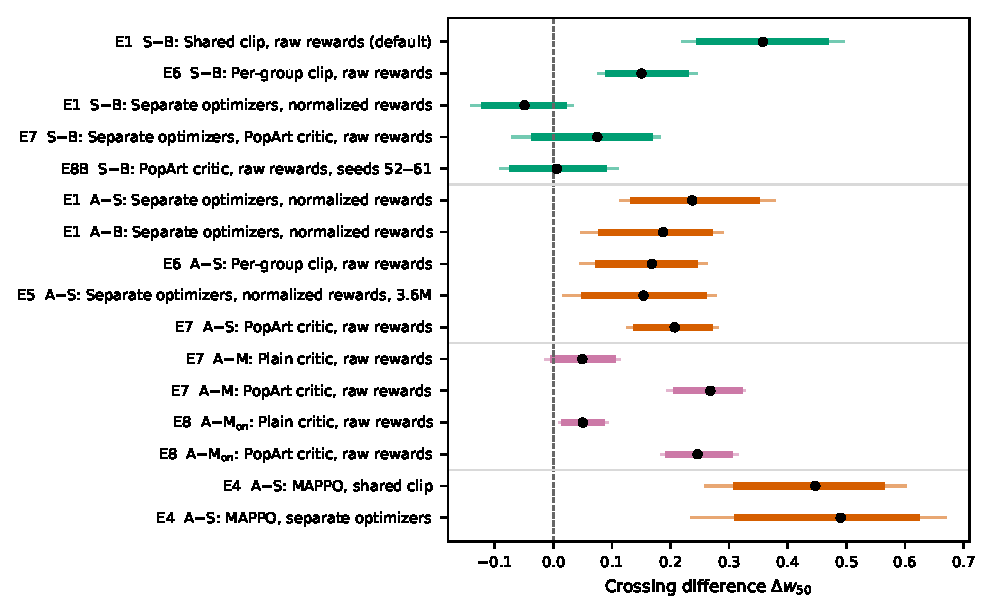
\includegraphics[width=\textwidth]{generated/v4/fig_summary.pdf}
\caption{Principal crossing contrasts across experiments. Thick bars: pre-declared 95\% seed-block intervals; thin bars: coverage-calibrated \VrvCalLevel{} intervals (Section~\ref{sec:stats}); dots: point estimates. Top block: symmetric scaling S$-$B under the default shared clip, per-group clipping, decoupled learner with normalized rewards, and PopArt critic. Middle: asymmetric contrasts on the supply chain. Lower: asymmetric versus the scale-matched symmetric control M, and the LBF replication.}
\label{fig:summary}
\Description{Dot-and-interval plot of thirteen contrasts; the default symmetric shift is large and positive, the decoupled and PopArt symmetric shifts include zero, asymmetric contrasts are positive, plain-critic A minus M touches zero.}
\end{figure}

\begin{table}[!htbp]
\caption{Evidence hierarchy for the optimizer account. Each level names the experiment that supports it and how far the evidence goes. ``Isolated'' means an intervention changes only the named quantity; ``consistent'' means the data agree with the explanation but an alternative is not excluded.}
\label{tab:hierarchy}
\centering\footnotesize
\begin{tabular}{@{}>{\raggedright\arraybackslash}p{.17\textwidth}>{\raggedright\arraybackslash}p{.40\textwidth}>{\raggedright\arraybackslash}p{.24\textwidth}>{\raggedright\arraybackslash}p{.11\textwidth}@{}}
\toprule
Level & Finding & Evidence & Status \\
\midrule
1. Observation & Under the default configuration, symmetric $\times7$ scaling moves the crossing (S$-$B \VfourSymStd{}). & E1, Table~\ref{tab:factorial_contrasts} & Direct \\
2. Diagnostic & The critic dominates the shared clip: pre-clip critic norm \VfourCriticNormB{} (B) vs.\ \VfourCriticNormS{} (S); the actor's applied gradient for S is \VsixGradGlobal{} of B's and its parameter update \VsixUpdGlobal{}. & E1, E6, Tables~\ref{tab:factorial_diagnostics} and~\ref{tab:e6} & Direct \\
3. Intervention & Clipping actor and critic separately restores the actor update (\VsixUpdGroup{}) and changes S$-$B by \VsixSymGroupChange{}. & E6 & Isolated \\
4. Residual & Without clipping S$-$B is \VfourSymSep{}; adding reward normalization gives \VfourSymBoth{} (\VfourSymNorm{} under the shared clip). & E1, E6 & Direct \\
5. Interpretation & Candidate: the residual reflects the critic's target scale. Normalizing only the critic's targets (PopArt) raises explained variance for S from \VsevenEVPlainS{} to \VsevenEVPopS{} (B: \VsevenEVPopB{}) and changes S$-$B by \VsevenSymChange{}. & E7, Table~\ref{tab:e7} & Tested, inconclusive \\
6. Moment control & A symmetric affine map of B matched to A's reward scale: A$-$M is \VsevenAMPlain{} with a raw-target critic and \VsevenAMPop{} with PopArt. Its SD matches A's; its mean is more negative. & E7, Table~\ref{tab:e7} & Raw targets: not separable; PopArt: direct \\
\bottomrule
\end{tabular}
\end{table}


\paragraph{Design (E1, E2).}
The pre-registered factorial crosses two optimizer modes with two reward modes at 300k. The optimizer
modes are SB3's default global clip and separate actor and critic Adam optimizers without clipping. The
reward modes are raw transformed rewards and online normalization (\texttt{VecNormalize} of rewards by
the running standard deviation of discounted returns, no observation normalization). Each cell runs the
four arms B, A, S and R on eight mixture cells $\{0,.2,.4,.5,.6,.7,.85,1\}$ with seeds 42--51, for
1,280 trajectories. An addendum (E2, 320 trajectories) keeps the default clip and raw rewards but sets
Adam's $\epsilon$ to $10^{-8}$. The pre-declared readings were: an A$-$S interval excluding zero after
both interventions indicates a sign-asymmetric effect; collapse of the symmetric contrasts after an
intervention indicates a scale or optimizer mechanism.

\paragraph{Prediction (a)--(b): under the shared clip, symmetric scaling mimics loss asymmetry.}
In the default cell every minibatch exceeds the clip norm, and the critic's pre-clip gradient norm
grows from \VfourCriticNormB{} (B) to \VfourCriticNormS{} (S) while the actor's stays near 2. The applied
actor update after clipping is \VfourAppliedActorB{} for B and \VfourAppliedActorS{} for S
(Table~\ref{tab:factorial_diagnostics}). Symmetric $\times7$ scaling therefore moves the crossing by
\VfourSymStd{} relative to B, at least as far as the loss multiplier, and A$-$S is
\VfourAsymStd{} (Table~\ref{tab:factorial_contrasts}).

\paragraph{Removing the coupling removes the detectable symmetric shift.}
With normalized rewards the critic's gradient falls below the clip norm, the actor carries almost all
of the gradient energy, and no symmetric shift is detectable (S$-$B \VfourSymNorm{}). With separate
optimizers alone the symmetric $\times7$ effect shrinks to \VfourSymSep{} and the $\times3.451$ effect is
no longer detectable. With both interventions, S$-$B is \VfourSymBoth{}. These intervals include zero, but
they are not equivalence results: under both interventions the interval extends beyond a $\pm.05$ margin, so
a symmetric shift of that size is not excluded. The changes in each contrast relative to the default cell are
in Table~\ref{tab:factorial_interactions}; Figure~\ref{fig:factorial} summarizes them.

\paragraph{The artifact is not Adam's $\epsilon$, and points to critic target magnitude.}
Lowering $\epsilon$ to $10^{-8}$ leaves the symmetric effect in place (S$-$B \VfourSymEps{}; change
relative to default \VfourSymEpsChange{}), contrary to our pre-declared alternative that the clipped
actor gradients were being suppressed by Adam's $\epsilon$ floor. Normalizing rewards, which bounds the
critic's targets, removes the detectable effect, whereas separating the optimizers only reduces it. The
critic's explained variance agrees: without clipping and with raw rewards it falls from
\VfourEVSepRawB{} (B) to \VfourEVSepRawS{} (S), whereas under reward normalization it is \VfourEVNormB{}
and \VfourEVNormS{}. Two qualifications limit this account. First, \texttt{VecNormalize} normalizes
rewards, not value targets as PopArt does~\citep{vanhasselt2016popart}; E7 and E8 below normalize the targets
alone. Second, the separate-optimizer
arm removes clipping as well; because Adam is per-parameter, splitting one Adam into two changes nothing
by itself, so this arm tests the removal of clipping, not optimizer grouping.

\paragraph{Prediction (c): clipping isolation (E6).}
A second pre-registered cohort (720 runs) clips actor and critic gradients separately under one Adam step,
and logs, at every optimizer step, both the applied gradient and the actual parameter change
(Table~\ref{tab:e6}). With logging switched on, the default and no-clip modes reproduce the corresponding
E1 runs exactly (\VsixRepro{} labels and profits), so the logging does not alter training. Under the shared
clip the actor's applied gradient for S is \VsixGradGlobal{} of B's, but Adam partly compensates, and the
actor's actual parameter update is \VsixUpdGlobal{} of B's. With per-group clipping or no clipping the ratio
is \VsixUpdGroup{} and \VsixUpdNone{}, close to but detectably below one, so our pre-declared prediction of
no difference is not met as stated. Per-group clipping reduces the symmetric effect by \VsixSymGroupChange{}
to \VsixSymGroup{}, and its crossings are almost identical to those without any clipping. The shared clip
therefore accounts for part of the artifact, roughly 0.2 of the 0.36 shift. The remainder is unaffected by
clipping, accompanies a poorly fitted critic, and disappears under reward normalization
(Section~\ref{sec:optimizer}, E1). The asymmetric contrast A$-$S is \VsixAsymGroup{} under per-group
clipping. Figure~\ref{fig:e6} puts the three steps side by side.

\begin{figure}[!htbp]
\centering
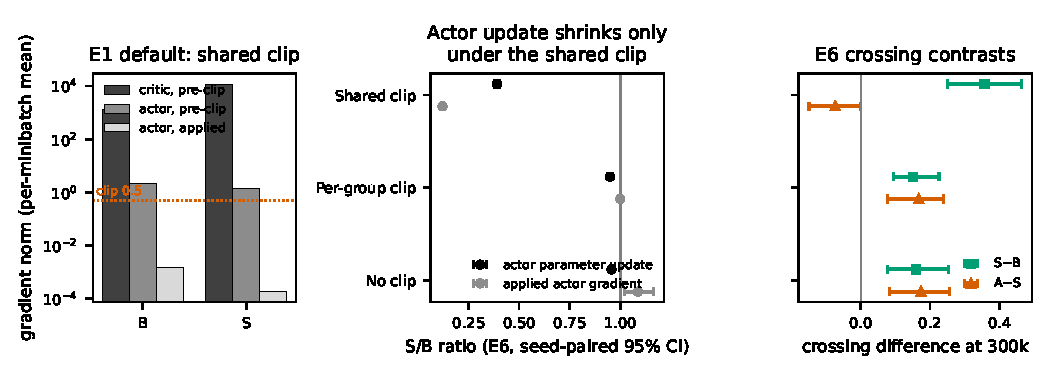
\includegraphics[width=\textwidth]{generated/v4/fig_e6_mechanism.pdf}
\caption{The shared-clip pathway. Left: in the default E1 cell (log scale) the critic's pre-clip gradient norm rises from \VrevCritB{} (B) to \VrevCritS{} (S) while the actor's stays near 2, so one global clip to 0.5 shrinks the actor's applied gradient more for S. Middle: E6 seed-paired S/B ratios of the actor's applied gradient and of its actual parameter update, with 95\% intervals; a parameter-update ratio is not a gradient ratio, because Adam rescales. Right: E6 crossing contrasts. Per-group clipping restores the actor update and removes part of the symmetric shift; A$-$S becomes positive.}
\label{fig:e6}
\Description{Three panels: bar chart of gradient norms on a log scale; dot plot of S over B ratios near 0.4 and 0.1 under the shared clip and near one otherwise; dot plot of crossing contrasts by clipping mode.}
\end{figure}

\paragraph{Prediction (d): critic-only target normalization (E7).}
Reward normalization rescales both the critic's targets and the rewards from which the actor's advantages
are built. E7 keeps separate optimizers without clipping and raw rewards, and crosses two critics with four
arms on the E1 grid (400 new runs; the plain-critic B, A and S runs are E1's, licensed by a gate that
reproduced an E1 run bit-for-bit). The \emph{plain} critic regresses raw returns. The \emph{PopArt} critic
reparametrizes its output as $V(x)=\sigma\,h(x)+\mu$, with $\mu,\sigma$ running moments of the rollout returns
and an output-preserving rescale of the head whenever they change~\citep{vanhasselt2016popart}; the actor's
rewards, advantages and loss are untouched. PopArt repairs the critic's fit: explained variance is
\VsevenEVPopB{} (B) and \VsevenEVPopS{} (S), against \VsevenEVPlainB{} and \VsevenEVPlainS{} with the plain
critic. The symmetric shift falls from \VsevenSymPlain{} to \VsevenSymPop{}, but the change, \VsevenSymChange{},
does not exclude zero. Our pre-declared criterion for attributing the residual to critic target scale required
both, so this reading is inconclusive: the point estimate is a partial reduction, and ten seeds cannot
separate it from none (Table~\ref{tab:e7}). A fresh cohort pre-registered after E7 (E8, seeds 52--61, both
critics, Table~\ref{tab:e8}) repeated the comparison. There the symmetric shift is \VeightBSymPlain{} with the
plain critic, replicating E7, and \VeightBSymPop{} with PopArt, and the change, \VeightBChange{}, excludes zero.
The pre-declared criterion is therefore met in the independent cohort, and the residual of prediction (d) is
attributed to critic target scale. The attribution rests on the declared 95\% intervals. At the
coverage-calibrated level the fresh cohort's change is \VeightBChangeNine{}, which includes zero; pooling both
cohorts, a secondary analysis declared in advance, gives \VeightPoolChange{} (\VeightPoolChangeNine{} at the
calibrated level).

\paragraph{The baseline crossing itself depends on the optimizer.}
The curvature-only crossing B is \VfourBaselineStd{} in the default cell and \VfourBaselineRange{} in
the other cells (Table~\ref{tab:factorial_crossings}). An absolute $\wcrit$ is therefore a property of
the learner's optimizer configuration as well as of the reward design; comparisons are valid only
within a fixed configuration.

\begin{table}[!htbp]
\caption{Optimizer $\times$ reward-normalization factorial (E1) and Adam-$\epsilon$ addendum (E2): crossings $w_{50}$ at 300k with 95\% seed-block intervals. B: curvature only; A: losses $\times7$; S: both branches $\times7$; R: both branches $\times3.451$ (A's pooled RMS ratio). Ten seeds per cell, eight mixture cells, one platform.}
\label{tab:factorial_crossings}
\centering\footnotesize
\begin{tabular}{@{}lcccc@{}}
\toprule
Optimizer / reward & B & A & S & R \\
\midrule
Global clip, raw (default) & \begin{tabular}[t]{@{}c@{}}$0.538$\\[-1pt]{\scriptsize $[0.461,\,0.624]$}\end{tabular} & \begin{tabular}[t]{@{}c@{}}$0.821$\\[-1pt]{\scriptsize $[0.775,\,0.864]$}\end{tabular} & \begin{tabular}[t]{@{}c@{}}$0.895$\\[-1pt]{\scriptsize $[0.835,\,0.957]$}\end{tabular} & \begin{tabular}[t]{@{}c@{}}$0.794$\\[-1pt]{\scriptsize $[0.775,\,0.821]$}\end{tabular} \\
Global clip, normalized reward & \begin{tabular}[t]{@{}c@{}}$0.306$\\[-1pt]{\scriptsize $[0.201,\,0.413]$}\end{tabular} & \begin{tabular}[t]{@{}c@{}}$0.593$\\[-1pt]{\scriptsize $[0.527,\,0.655]$}\end{tabular} & \begin{tabular}[t]{@{}c@{}}$0.356$\\[-1pt]{\scriptsize $[0.272,\,0.436]$}\end{tabular} & \begin{tabular}[t]{@{}c@{}}$0.367$\\[-1pt]{\scriptsize $[0.324,\,0.414]$}\end{tabular} \\
Separate optimizers, raw & \begin{tabular}[t]{@{}c@{}}$0.326$\\[-1pt]{\scriptsize $[0.256,\,0.392]$}\end{tabular} & \begin{tabular}[t]{@{}c@{}}$0.661$\\[-1pt]{\scriptsize $[0.628,\,0.696]$}\end{tabular} & \begin{tabular}[t]{@{}c@{}}$0.487$\\[-1pt]{\scriptsize $[0.412,\,0.569]$}\end{tabular} & \begin{tabular}[t]{@{}c@{}}$0.353$\\[-1pt]{\scriptsize $[0.270,\,0.442]$}\end{tabular} \\
Separate optimizers, normalized & \begin{tabular}[t]{@{}c@{}}$0.414$\\[-1pt]{\scriptsize $[0.351,\,0.506]$}\end{tabular} & \begin{tabular}[t]{@{}c@{}}$0.602$\\[-1pt]{\scriptsize $[0.560,\,0.641]$}\end{tabular} & \begin{tabular}[t]{@{}c@{}}$0.365$\\[-1pt]{\scriptsize $[0.282,\,0.439]$}\end{tabular} & \begin{tabular}[t]{@{}c@{}}$0.350$\\[-1pt]{\scriptsize $[0.252,\,0.438]$}\end{tabular} \\
Global clip, raw, Adam $\epsilon{=}10^{-8}$ & \begin{tabular}[t]{@{}c@{}}$0.450$\\[-1pt]{\scriptsize $[0.387,\,0.534]$}\end{tabular} & \begin{tabular}[t]{@{}c@{}}$0.757$\\[-1pt]{\scriptsize $[0.729,\,0.775]$}\end{tabular} & \begin{tabular}[t]{@{}c@{}}$0.708$\\[-1pt]{\scriptsize $[0.649,\,0.770]$}\end{tabular} & \begin{tabular}[t]{@{}c@{}}$0.615$\\[-1pt]{\scriptsize $[0.559,\,0.683]$}\end{tabular} \\
\bottomrule
\end{tabular}
\end{table}

\begin{table}[t]
\caption{Paired seed-block contrasts within each optimizer cell. $^{\ast}$: 95\% interval excludes zero. A$-$S is the pre-declared asymmetry contrast; S$-$B and R$-$B are symmetric-scaling effects.}
\label{tab:factorial_contrasts}
\centering\scriptsize
\resizebox{\linewidth}{!}{%
\begin{tabular}{@{}lcccc@{}}
\toprule
Optimizer / reward & A$-$S & A$-$B & S$-$B & R$-$B \\
\midrule
Global clip, raw (default) & $-0.074$ $[-0.150,\,+0.000]$ & $+0.283$$^{\ast}$ $[+0.181,\,+0.386]$ & $+0.357$$^{\ast}$ $[+0.249,\,+0.464]$ & $+0.256$$^{\ast}$ $[+0.160,\,+0.344]$ \\
Global clip, normalized reward & $+0.237$$^{\ast}$ $[+0.169,\,+0.305]$ & $+0.287$$^{\ast}$ $[+0.199,\,+0.386]$ & $+0.050$ $[-0.035,\,+0.144]$ & $+0.060$ $[-0.068,\,+0.179]$ \\
Separate optimizers, raw & $+0.174$$^{\ast}$ $[+0.083,\,+0.255]$ & $+0.334$$^{\ast}$ $[+0.274,\,+0.405]$ & $+0.160$$^{\ast}$ $[+0.078,\,+0.254]$ & $+0.027$ $[-0.024,\,+0.069]$ \\
Separate optimizers, normalized & $+0.237$$^{\ast}$ $[+0.136,\,+0.346]$ & $+0.188$$^{\ast}$ $[+0.082,\,+0.266]$ & $-0.049$ $[-0.117,\,+0.017]$ & $-0.064$ $[-0.176,\,+0.024]$ \\
Global clip, raw, Adam $\epsilon{=}10^{-8}$ & $+0.048$ $[-0.013,\,+0.111]$ & $+0.307$$^{\ast}$ $[+0.224,\,+0.363]$ & $+0.258$$^{\ast}$ $[+0.187,\,+0.330]$ & $+0.165$$^{\ast}$ $[+0.109,\,+0.219]$ \\
\bottomrule
\end{tabular}
}
\end{table}

\begin{table}[!htbp]
\caption{Clipping isolation (E6): one Adam step with a global clip, actor and critic clipped separately, or no clipping; raw rewards; arms B, A, S on the E1 grid; ten seeds; 720 runs at 300k. Crossing contrasts, and seed-paired S/B ratios of the actor's applied (post-clip) gradient norm and of the norm of its actual parameter update. $^{\ast}$: interval excludes zero.}
\label{tab:e6}
\centering\footnotesize
\begin{tabular}{@{}lcccc@{}}
\toprule
Mode & S$-$B & A$-$S & Applied actor gradient S/B & Actor update S/B \\
\midrule
Global clip (default) & \begin{tabular}[t]{@{}c@{}}$+0.357$$^{\ast}$\\[-1pt]{\scriptsize $[+0.249,\,+0.464]$}\end{tabular} & \begin{tabular}[t]{@{}c@{}}$-0.074$\\[-1pt]{\scriptsize $[-0.150,\,+0.000]$}\end{tabular} & \begin{tabular}[t]{@{}c@{}}$0.121$\\[-1pt]{\scriptsize $[0.114,\,0.129]$}\end{tabular} & \begin{tabular}[t]{@{}c@{}}$0.391$\\[-1pt]{\scriptsize $[0.378,\,0.405]$}\end{tabular} \\
Per-group clip & \begin{tabular}[t]{@{}c@{}}$+0.150$$^{\ast}$\\[-1pt]{\scriptsize $[+0.095,\,+0.226]$}\end{tabular} & \begin{tabular}[t]{@{}c@{}}$+0.168$$^{\ast}$\\[-1pt]{\scriptsize $[+0.077,\,+0.240]$}\end{tabular} & \begin{tabular}[t]{@{}c@{}}$1.000$\\[-1pt]{\scriptsize $[1.000,\,1.000]$}\end{tabular} & \begin{tabular}[t]{@{}c@{}}$0.949$\\[-1pt]{\scriptsize $[0.936,\,0.962]$}\end{tabular} \\
No clip & \begin{tabular}[t]{@{}c@{}}$+0.160$$^{\ast}$\\[-1pt]{\scriptsize $[+0.078,\,+0.254]$}\end{tabular} & \begin{tabular}[t]{@{}c@{}}$+0.174$$^{\ast}$\\[-1pt]{\scriptsize $[+0.083,\,+0.255]$}\end{tabular} & \begin{tabular}[t]{@{}c@{}}$1.087$\\[-1pt]{\scriptsize $[1.021,\,1.164]$}\end{tabular} & \begin{tabular}[t]{@{}c@{}}$0.956$\\[-1pt]{\scriptsize $[0.944,\,0.967]$}\end{tabular} \\
\bottomrule
\end{tabular}
\end{table}


\begin{figure}[!htbp]
\centering
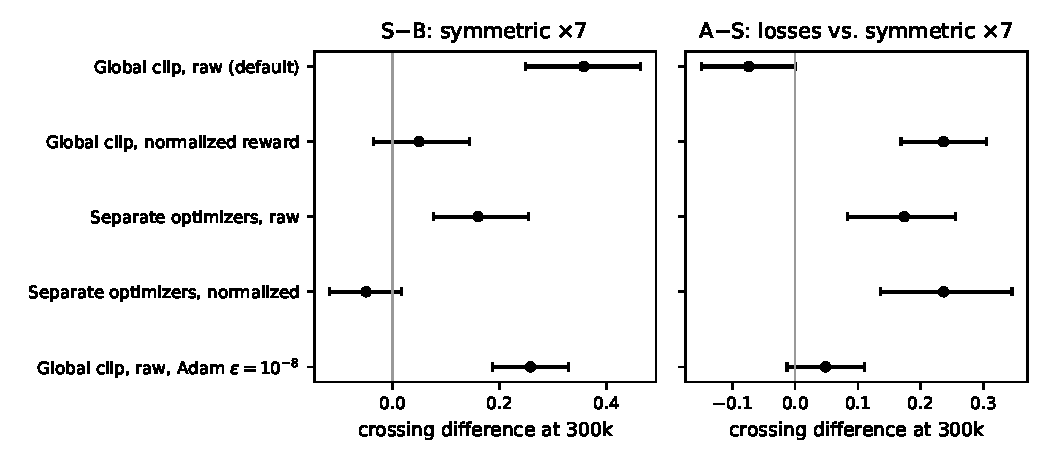
\includegraphics[width=\textwidth]{generated/v4/factorial_contrasts.pdf}
\caption{Symmetric-scaling (left) and asymmetric-minus-symmetric (right) crossing differences in each optimizer cell, with paired 95\% seed-block intervals. Under the default configuration (top row) symmetric scaling moves the crossing as far as the loss multiplier; with normalized rewards and/or separate optimizers it does not, while A$-$S becomes positive.}
\label{fig:factorial}
\Description{Two dot-and-interval panels across five optimizer cells. Symmetric effects are large in the default cell and near zero under normalization; asymmetric-minus-symmetric differences are near zero by default and positive under the interventions.}
\end{figure}

\begin{table}[!htbp]
\caption{Critic-target normalization and a moment-matched control (E7): separate actor and critic optimizers without clipping, raw rewards, the E1 grid, ten seeds, 300k. M is the affine map $a_w r_{\mathrm{B}}+b_w$ of B's reward with constants frozen to give A's E1 training-reward mean and SD. The plain-critic B, A and S runs are E1's. Crossing contrasts with paired 95\% seed-block intervals; the bottom row is the change in each contrast from the plain to the PopArt critic. $^{\ast}$: interval excludes zero.}
\label{tab:e7}
\centering\footnotesize
\begin{tabular}{@{}lccccc@{}}
\toprule
Critic & S$-$B & A$-$S & A$-$M & M$-$B & A$-$B \\
\midrule
Plain & \begin{tabular}[t]{@{}c@{}}$+0.160$$^{\ast}$\\[-1pt]{\scriptsize $[+0.078,\,+0.254]$}\end{tabular} & \begin{tabular}[t]{@{}c@{}}$+0.174$$^{\ast}$\\[-1pt]{\scriptsize $[+0.083,\,+0.255]$}\end{tabular} & \begin{tabular}[t]{@{}c@{}}$+0.050$\\[-1pt]{\scriptsize $[+0.000,\,+0.100]$}\end{tabular} & \begin{tabular}[t]{@{}c@{}}$+0.285$$^{\ast}$\\[-1pt]{\scriptsize $[+0.208,\,+0.363]$}\end{tabular} & \begin{tabular}[t]{@{}c@{}}$+0.334$$^{\ast}$\\[-1pt]{\scriptsize $[+0.274,\,+0.405]$}\end{tabular} \\
PopArt & \begin{tabular}[t]{@{}c@{}}$+0.075$\\[-1pt]{\scriptsize $[-0.032,\,+0.164]$}\end{tabular} & \begin{tabular}[t]{@{}c@{}}$+0.207$$^{\ast}$\\[-1pt]{\scriptsize $[+0.141,\,+0.266]$}\end{tabular} & \begin{tabular}[t]{@{}c@{}}$+0.268$$^{\ast}$\\[-1pt]{\scriptsize $[+0.211,\,+0.317]$}\end{tabular} & \begin{tabular}[t]{@{}c@{}}$+0.014$\\[-1pt]{\scriptsize $[-0.082,\,+0.113]$}\end{tabular} & \begin{tabular}[t]{@{}c@{}}$+0.282$$^{\ast}$\\[-1pt]{\scriptsize $[+0.181,\,+0.380]$}\end{tabular} \\
PopArt$-$plain & \begin{tabular}[t]{@{}c@{}}$-0.085$\\[-1pt]{\scriptsize $[-0.183,\,+0.006]$}\end{tabular} & \begin{tabular}[t]{@{}c@{}}$+0.033$\\[-1pt]{\scriptsize $[-0.080,\,+0.135]$}\end{tabular} & \begin{tabular}[t]{@{}c@{}}$+0.218$$^{\ast}$\\[-1pt]{\scriptsize $[+0.143,\,+0.298]$}\end{tabular} &  &  \\
\bottomrule
\end{tabular}
\end{table}


% =======================================================================

\FloatBarrier

\section{Asymmetric Reward Transforms}
\label{sec:asymmetric}

\paragraph{The loss multiplier opposes curvature.}
In the legacy decomposition at 300k (20 seeds per cell), the linear null gives \RepeatedNull{}; this is a
separate run from the structural sweep of Section~\ref{sec:robustness} (\Headline{}), with a different
$w$-grid, and the decomposition uses its own null. Curvature
alone ($\alpha{=}\beta{=}0.88$, the conventional prospect-theory estimate~\citep{tversky1992}, not tuned)
lowers the crossing to 0.585 ($-0.100$ $[-0.145,-0.057]$ vs.\ linear), and raising $\lambda$ from 1 to 7
raises it to \HighLambda{} (Figure~\ref{fig:decomposition}; per-$\lambda$ values in
Appendix~\ref{app:estimation}). Reported as a single ``prospect-theoretic'' treatment the two effects
partially cancel. Against the curvature baseline the loss-multiplier shift is \LossMultiplierShift{}.
On its own, this shift cannot distinguish loss asymmetry from the larger reward magnitude the multiplier
creates; Section~\ref{sec:optimizer} showed how; this section separates the two.

\begin{figure}[!htbp]
\centering
\includegraphics[width=.74\textwidth]{generated/decomposition_observed.pdf}
\caption{Legacy supply PPO null and selected transform conditions at 300k. Points show collapse counts divided by cell totals with 95\% Wilson intervals; curves are Firth fits over observed grids. Vertical bands are midpoint seed-block intervals.}
\label{fig:decomposition}
\Description{Four panels compare observed collapse proportions and fitted midpoints for null, lambda one, lambda three and lambda seven.}
\end{figure}

\begin{table*}[t]
\caption{Supply-PPO reward-transform decomposition at 300k requested agent transitions and descriptive equivalent linear-training budgets. Differences use paired seed-block draws. Equivalent budgets invert the four-point cross-sectional fit $w_{50}=1.4824-0.13748\ln(T/1000)$ and propagate the same 2,000 bootstrap replicates; they are descriptive, not causal. $\dagger$ denotes extrapolation below the observed 150k--900k horizon range.}
\label{tab:decomposition}
\centering\small
{\setlength{\tabcolsep}{4pt}
\begin{tabular}{@{}lllll@{}}
\toprule
Condition & Crossing and 95\% CI & Versus null & Versus curvature & Equivalent budget, k \\
\midrule
Linear null & $0.685$ $[0.650,0.715]$ & -- & -- & $330$ $[275,406]$ \\
Curvature ($\lambda=1$) & $0.585$ $[0.544,0.624]$ & $-0.100$ $[-0.145,-0.057]$ & -- & $685$ $[535,942]$ \\
$\lambda=3$ & $0.775$ $[0.755,0.790]$ & $+0.090$ $[+0.065,+0.115]$ & $+0.190$ $[+0.150,+0.229]$ & $172$ $[140,211]$ \\
$\lambda=7$ & $0.852$ $[0.840,0.865]$ & $+0.167$ $[+0.134,+0.203]$ & $+0.268$ $[+0.230,+0.306]$ & $98$ $[67,128]$$^{\dagger}$ \\
\bottomrule
\end{tabular}
}
\end{table*}


\paragraph{Equivalent linear-training budget.}
As a descriptive translation, inverting the legacy cross-sectional fit
$w_{50}=1.4824-0.13748\ln(T/1000)$ maps curvature-only at 300k to a linear budget of 685k $[535,942]$
and $\lambda=7$ to 98k $[67,128]$ (an extrapolation below the observed 150k--900k range); the repeated
linear null maps to 330k $[275,406]$ (Table~\ref{tab:decomposition}). This mapping is not causal,
and it is consistent with Section~\ref{sec:optimizer}: under the default optimizer the loss multiplier
behaves like a smaller training budget.

\paragraph{With the coupling removed, the loss multiplier still moves the crossing (E1, E6).}
Because A and S apply the same multiplier to losses and differ only in whether gains are also scaled, A$-$S
compares two gain-to-loss ratios (1:7 and 1:1) at matched loss scale, and A$-$B isolates the loss-branch
multiplier at fixed gains. A$-$S is positive and excludes zero under normalization (\VfourAsymNorm{}),
separate optimizers (\VfourAsymSep{}), both together (\VfourAsymBoth{}) and per-group clipping
(\VsixAsymGroup{}), and A$-$B is \VfourLossBoth{} with both interventions, so the pre-declared criterion for a
sign-asymmetric effect is met. How much of each reward falls on the loss branch depends on $w$ and on the
learned policy, because $z_0$ is fixed; near the crossings both branches are active
(Table~\ref{tab:loss_occupancy}). The arms also differ in reward mean, not only in scale: A's transformed
rewards have a negative mean at most $w$, whereas S and R have positive means that grow with $w$
(Figure~\ref{fig:reward_moments}, Appendix~\ref{app:factorial}). A$-$S therefore compares gain-to-loss ratios
but does not hold the first two moments fixed.

\paragraph{The asymmetric contrast persists with budget (E5).}
To test the asymmetric effect over budget without the scale pathway, we repeated the horizon design with
the fully decoupled learner of Section~\ref{sec:optimizer} (separate optimizers without clipping,
normalized rewards) and arms B, A and S: 270 trajectories on the same nine cells to 3.6M. All three
pre-declared predictions are met (Table~\ref{tab:e5}). A$-$S is positive at every primary budget, from
\VfiveAsymStart{} at 300k to \VfiveAsymEnd{} at 3.6M, and no symmetric shift is detectable at any budget
(S$-$B \VfiveSymStart{} at 300k, \VfiveSymEnd{} at 3.6M). The loss-only contrast A$-$B is positive to
900k and not detectable afterwards. Under this learner the crossings fall to 900k and then rise as many
initially coordinated trajectories relapse into collapse, and no arm stabilizes. The asymmetric effect
therefore persists over the tested budgets while the absolute crossings keep moving.
Figure~\ref{fig:e5} shows all 24 checkpoints. This reading of the non-primary checkpoints is exploratory
and its intervals are pointwise. The A$-$S interval excludes zero at \VrevAsymPos{} checkpoints, with
point estimates between \VrevAsymMin{} and \VrevAsymMax{}. The S$-$B interval excludes zero at
\VrevSymNeg{} intermediate checkpoints (\VrevSymNegSpan{}), all with S \emph{below} B, and at no
checkpoint with S above B. The default-optimizer E3 contrast is drawn for comparison; its own crossings
are in Figure~\ref{fig:horizon} (Appendix~\ref{app:horizon}).

\begin{table}[!htbp]
\caption{Decoupled horizon cohort (E5): separate actor and critic optimizers without clipping and normalized rewards; arms B, A, S; the nine E3 cells; ten seeds; 270 trajectories to 3.6M. Crossings, then paired contrasts. $^{\ast}$: interval excludes zero.}
\label{tab:e5}
\centering\footnotesize
\begin{tabular}{@{}lcccc@{}}
\toprule
Arm or contrast & 300k & 900k & 1.8M & 3.6M \\
\midrule
B (curvature) & \begin{tabular}[t]{@{}c@{}}$0.425$\\[-1pt]{\scriptsize $[0.344,\,0.507]$}\end{tabular} & \begin{tabular}[t]{@{}c@{}}$0.385$\\[-1pt]{\scriptsize $[0.332,\,0.439]$}\end{tabular} & \begin{tabular}[t]{@{}c@{}}$0.639$\\[-1pt]{\scriptsize $[0.541,\,0.715]$}\end{tabular} & \begin{tabular}[t]{@{}c@{}}$0.732$\\[-1pt]{\scriptsize $[0.638,\,0.866]$}\end{tabular} \\
A (losses $\times7$) & \begin{tabular}[t]{@{}c@{}}$0.603$\\[-1pt]{\scriptsize $[0.564,\,0.640]$}\end{tabular} & \begin{tabular}[t]{@{}c@{}}$0.526$\\[-1pt]{\scriptsize $[0.452,\,0.597]$}\end{tabular} & \begin{tabular}[t]{@{}c@{}}$0.667$\\[-1pt]{\scriptsize $[0.612,\,0.731]$}\end{tabular} & \begin{tabular}[t]{@{}c@{}}$0.837$\\[-1pt]{\scriptsize $[0.766,\,0.916]$}\end{tabular} \\
S (both $\times7$) & \begin{tabular}[t]{@{}c@{}}$0.369$\\[-1pt]{\scriptsize $[0.267,\,0.450]$}\end{tabular} & \begin{tabular}[t]{@{}c@{}}$0.329$\\[-1pt]{\scriptsize $[0.237,\,0.391]$}\end{tabular} & \begin{tabular}[t]{@{}c@{}}$0.548$\\[-1pt]{\scriptsize $[0.427,\,0.646]$}\end{tabular} & \begin{tabular}[t]{@{}c@{}}$0.683$\\[-1pt]{\scriptsize $[0.592,\,0.759]$}\end{tabular} \\
A$-$S & \begin{tabular}[t]{@{}c@{}}$+0.234$$^{\ast}$\\[-1pt]{\scriptsize $[+0.165,\,+0.322]$}\end{tabular} & \begin{tabular}[t]{@{}c@{}}$+0.197$$^{\ast}$\\[-1pt]{\scriptsize $[+0.086,\,+0.328]$}\end{tabular} & \begin{tabular}[t]{@{}c@{}}$+0.119$$^{\ast}$\\[-1pt]{\scriptsize $[+0.034,\,+0.244]$}\end{tabular} & \begin{tabular}[t]{@{}c@{}}$+0.154$$^{\ast}$\\[-1pt]{\scriptsize $[+0.053,\,+0.256]$}\end{tabular} \\
A$-$B & \begin{tabular}[t]{@{}c@{}}$+0.178$$^{\ast}$\\[-1pt]{\scriptsize $[+0.081,\,+0.271]$}\end{tabular} & \begin{tabular}[t]{@{}c@{}}$+0.141$$^{\ast}$\\[-1pt]{\scriptsize $[+0.064,\,+0.224]$}\end{tabular} & \begin{tabular}[t]{@{}c@{}}$+0.028$\\[-1pt]{\scriptsize $[-0.044,\,+0.113]$}\end{tabular} & \begin{tabular}[t]{@{}c@{}}$+0.105$\\[-1pt]{\scriptsize $[-0.045,\,+0.242]$}\end{tabular} \\
S$-$B & \begin{tabular}[t]{@{}c@{}}$-0.056$\\[-1pt]{\scriptsize $[-0.147,\,+0.043]$}\end{tabular} & \begin{tabular}[t]{@{}c@{}}$-0.056$\\[-1pt]{\scriptsize $[-0.146,\,+0.016]$}\end{tabular} & \begin{tabular}[t]{@{}c@{}}$-0.091$\\[-1pt]{\scriptsize $[-0.262,\,+0.054]$}\end{tabular} & \begin{tabular}[t]{@{}c@{}}$-0.049$\\[-1pt]{\scriptsize $[-0.240,\,+0.099]$}\end{tabular} \\
\bottomrule
\end{tabular}
\end{table}


\begin{figure}[!htbp]
\centering
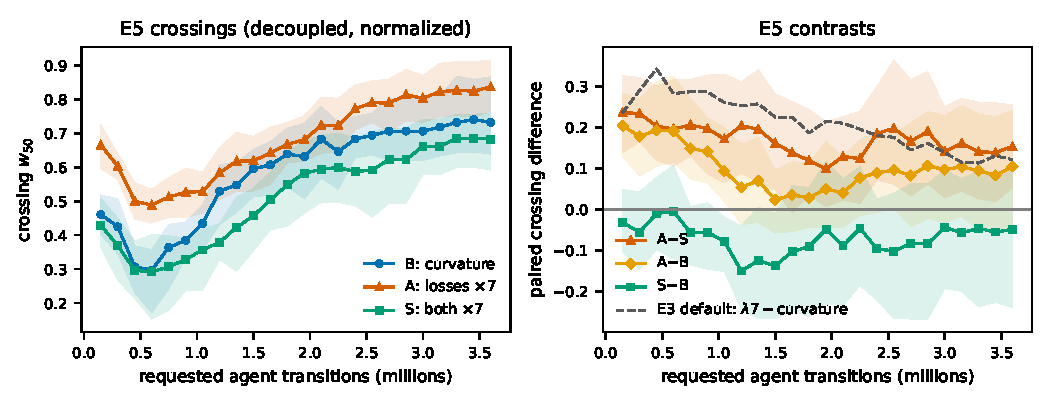
\includegraphics[width=\textwidth]{generated/v4/fig_e5_horizon.pdf}
\caption{Decoupled horizon cohort (E5) at all 24 checkpoints. Left: crossings of B, A and S with pointwise 95\% seed-block bands. Right: paired contrasts with bands; the dashed line is the default-optimizer E3 contrast $\lambda7-$curvature (the E3 analogue of A$-$B, which includes the scale pathway). Nine mixture cells, ten seeds per cell and arm.}
\label{fig:e5}
\Description{Left: three crossing curves falling to about 600k and rising to 3.6M, with A highest throughout. Right: A minus S stays above zero at every checkpoint; S minus B stays near or below zero.}
\end{figure}

\paragraph{Against a scale-matched symmetric control, the effect depends on the critic (E7).}
E7's arm M is an increasing affine map $a_w r_{\mathrm{B}}+b_w$ of B's reward, symmetric in gains and losses,
with constants frozen so that M has A's E1 training-reward mean and SD. With the plain critic, M moves the
crossing by \VsevenMBPlain{} relative to B, most of A's \VsevenABPlain{}, and A$-$M is \VsevenAMPlain{}; its
lower bound touches zero (\VrvPlainAMcal{} at the calibrated level), so the pre-declared prediction that A
exceeds M under both critics is not met. On E7 alone, therefore, the A$-$S contrast under a raw-target critic
could be an effect of the reward's moments rather than of its sign asymmetry; E8 below tests this. With the PopArt critic M is
indistinguishable from B (\VsevenMBPop{}), while A exceeds both S (\VsevenAsymPop{}) and M (\VsevenAMPop{});
the change in A$-$M between critics is \VsevenAMChange{}.

One qualification applies to both readings (Figure~\ref{fig:e7_moments}). The affine constants match A's
moments under E1's policies, but M's achieved moments depend on its own: M matches A's SD
(\VsevenSDPlainM{} vs.\ \VsevenSDPlainA{} with the plain critic, \VsevenSDPopM{} vs.\ \VsevenSDPopA{} with
PopArt) but not its mean (\VsevenMeanPlainM{} vs.\ \VsevenMeanPlainA{}; \VsevenMeanPopM{} vs.\
\VsevenMeanPopA{}), failing the pre-declared 25\% matching check. The mismatch is concentrated at
$w\in[0.4,0.7]$. There M's policies, like A's, mostly collapse, whereas the B policies whose moments set M's
constants mostly do not, and B's reward is lower under a collapsed policy. M is
thus a scale-matched control whose mean is more negative than A's, and the plain-critic reading cannot
separate a moment effect from that mean difference. An affine control can match at most the first two
moments; what it leaves different, by construction, is the shape of the reward distribution, which is the
feature an asymmetric transform is meant to change. The training-reward logs confirm this and show one further
difference (Table~\ref{tab:dist}, Appendix~\ref{app:factorial}). A's per-rollout reward is left-skewed (quantile
skewness \VdaSkewA{}), M's is not (\VdaSkewM{}). With the plain critic, M's critic targets are also larger than
A's (mean return \VdaRetMeanM{} against \VdaRetMeanA{}, SD \VdaRetSdM{} against \VdaRetSdA{}). Larger target
scale is the pathway with which the residual symmetric shift is consistent (Section~\ref{sec:optimizer}), so with
a raw-target critic M is exposed to it at least as much as A. This is consistent with, but does not establish, a
target-scale explanation of the near-null plain-critic A$-$M.

\paragraph{An online moment-matched control separates moments from shape (E8).}
E8's control M$_{\mathrm{on}}$ applies the same kind of increasing affine map to B's reward, but re-sets its
constants before every rollout. They are chosen so that its training-reward mean and SD track A's, rollout by
rollout, under M$_{\mathrm{on}}$'s own policy; the targets are the seed-averaged per-rollout moments of A in the
same critic mode, frozen before any E8 run. The matching criterion is met. Pooled over the eight cells, M$_{\mathrm{on}}$'s
achieved mean and SD lie within \VeightMatchMeanPlain{} and \VeightMatchSdPlain{} of A's with the plain critic,
and within \VeightMatchMeanPop{} and \VeightMatchSdPop{} with PopArt; \VeightClamp{} of \VeightNA{} runs
reached the declared lower bound on the scale at some rollout. Matching the mean leaves the control where it
was: M$_{\mathrm{on}}-$M is \VeightMonMPlain{} (plain) and \VeightMonMPop{} (PopArt), so E7's mean mismatch was
not driving its result. With PopArt, A$-$M$_{\mathrm{on}}$ is \VeightAMonPop{}. With the plain critic it is
\VeightAMonPlain{}, and it also excludes zero at the calibrated level (\VeightAMonPlainNine{}). By the
pre-declared rule, the plain-critic asymmetric contrast is therefore not explained by the training reward's first
two moments, and the E7 reading above is revised. The part that is not explained is small, however.
M$_{\mathrm{on}}-$B is \VeightMonBPlain{}, most of A$-$B (\VsevenABPlain{}). So with a raw-target critic, most of
the loss-only shift is reproduced by a symmetric reward with the same moments; only the remainder,
A$-$M$_{\mathrm{on}}$, depends on the asymmetric shape. With PopArt the moment-matched symmetric control has no detectable effect
(\VeightMonBPop{}), and the asymmetric effect is large. Two features of the design limit this reading.
M$_{\mathrm{on}}$'s map changes between rollouts whereas A's is fixed. And an affine control matches only the first
two moments, so A$-$M$_{\mathrm{on}}$ contrasts A with a moment-matched, nonstationary symmetric control, not a
manipulation of sign asymmetry alone.

\begin{table}[!htbp]
\caption{Online moment-matched control and fresh-seed replication (E8): separate optimizers without clipping, raw rewards, the E1 grid, 300k. Top: M$_{\mathrm{on}}$ is an affine map of B's reward whose constants are reset every rollout so that its training-reward mean and SD track A's under its own policy; A, B, S and the static control M are the E1 and E7 runs on the same seeds (42--51). Bottom: S$-$B with fresh seeds 52--61 (pre-declared primary) and pooled with E1/E7's seeds 42--51 (secondary), and its change from the plain to the PopArt critic. Paired 95\% seed-block intervals; $^{\ast}$: interval excludes zero.}
\label{tab:e8}
\centering\footnotesize
\begin{tabular}{@{}lcccc@{}}
\toprule
Critic & A$-$M$_{\mathrm{on}}$ & M$_{\mathrm{on}}-$B & M$_{\mathrm{on}}-$M & A$-$S \\
\midrule
Plain & \begin{tabular}[t]{@{}c@{}}$+0.050$$^{\ast}$\\[-1pt]{\scriptsize $[+0.020,\,+0.082]$}\end{tabular} & \begin{tabular}[t]{@{}c@{}}$+0.284$$^{\ast}$\\[-1pt]{\scriptsize $[+0.234,\,+0.338]$}\end{tabular} & \begin{tabular}[t]{@{}c@{}}$-0.001$\\[-1pt]{\scriptsize $[-0.051,\,+0.049]$}\end{tabular} & \begin{tabular}[t]{@{}c@{}}$+0.174$$^{\ast}$\\[-1pt]{\scriptsize $[+0.083,\,+0.255]$}\end{tabular} \\
PopArt & \begin{tabular}[t]{@{}c@{}}$+0.246$$^{\ast}$\\[-1pt]{\scriptsize $[+0.197,\,+0.300]$}\end{tabular} & \begin{tabular}[t]{@{}c@{}}$+0.036$\\[-1pt]{\scriptsize $[-0.066,\,+0.130]$}\end{tabular} & \begin{tabular}[t]{@{}c@{}}$+0.022$\\[-1pt]{\scriptsize $[-0.046,\,+0.085]$}\end{tabular} & \begin{tabular}[t]{@{}c@{}}$+0.207$$^{\ast}$\\[-1pt]{\scriptsize $[+0.141,\,+0.266]$}\end{tabular} \\
\midrule
Cohort & Plain S$-$B & PopArt S$-$B & Change, PopArt$-$plain & \\
\midrule
Seeds 52--61 (primary) & \begin{tabular}[t]{@{}c@{}}$+0.162$$^{\ast}$\\[-1pt]{\scriptsize $[+0.058,\,+0.262]$}\end{tabular} & \begin{tabular}[t]{@{}c@{}}$+0.006$\\[-1pt]{\scriptsize $[-0.070,\,+0.085]$}\end{tabular} & \begin{tabular}[t]{@{}c@{}}$-0.156$$^{\ast}$\\[-1pt]{\scriptsize $[-0.303,\,-0.016]$}\end{tabular} \\
Seeds 42--61 (secondary) & \begin{tabular}[t]{@{}c@{}}$+0.159$$^{\ast}$\\[-1pt]{\scriptsize $[+0.094,\,+0.231]$}\end{tabular} & \begin{tabular}[t]{@{}c@{}}$+0.044$\\[-1pt]{\scriptsize $[-0.021,\,+0.109]$}\end{tabular} & \begin{tabular}[t]{@{}c@{}}$-0.115$$^{\ast}$\\[-1pt]{\scriptsize $[-0.209,\,-0.032]$}\end{tabular} \\
\bottomrule
\end{tabular}
\end{table}


\begin{figure}[!htbp]
\centering
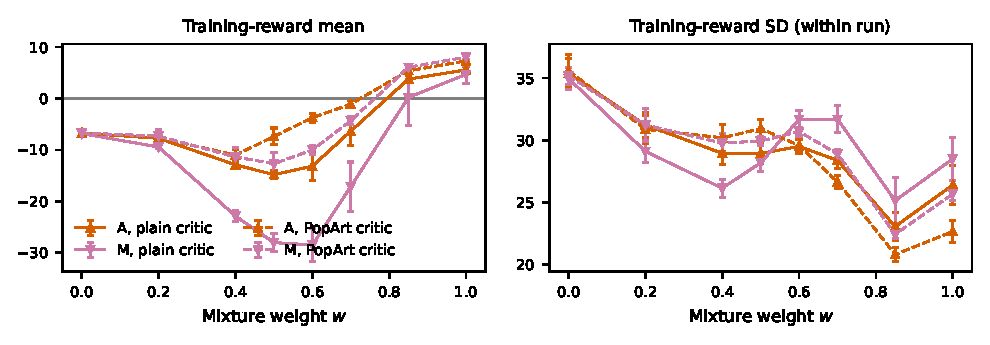
\includegraphics[width=\textwidth]{generated/v4/fig_e7_moments.pdf}
\caption{Achieved training-reward moments of the loss-multiplier arm A and the scale-matched symmetric control M in E7, by mixture weight (mean over ten seeds; bars are $\pm1.96$ standard errors across seeds). M matches A's within-run SD closely but its mean falls below A's at middle weights, most with the plain critic: there M's policies mostly collapse, unlike the B policies whose moments set its constants. The plain-critic A runs are E1's.}
\label{fig:e7_moments}
\Description{Two panels against mixture weight. Left: mean training reward, with M under the plain critic dropping to about minus 28 at middle weights while A stays near minus 13. Right: within-run SD, similar for A and M.}
\end{figure}

% =======================================================================

\FloatBarrier

\FloatBarrier
\section{A Second Environment: Level-Based Foraging}
\label{sec:lbf}

\paragraph{Design (E4).}
We repeated the arm comparison with centralized-critic MAPPO~\citep{yu2022surprising} on Level-Based
Foraging~\citep{christianos2020shared} (5$\times$5 grid, two players, two foods), using the same SB3
update with a global clip or with separate optimizers. The local reward is the native food share minus
an effort cost of 0.02 per LOAD attempt; the team reward sums native food rewards; collapse is a native
team return below $\theta=0.626$ over ten evaluation episodes, the midpoint between collapsed and coordinated team returns in an earlier calibration; the evaluation never includes the effort cost. The arms are
linear, curvature only, A ($\lambda=4$) and S (both branches $\times4$), on ten mixture cells with ten
seeds and 2M timesteps (800 trajectories).

\paragraph{The asymmetric contrast replicates under both optimizers.}
A raises the crossing relative to S by \VfourLBFAsymGlobal{} with the global clip and \VfourLBFAsymSep{}
with separate optimizers, and relative to curvature only by \VfourLBFLossOnlyGlobal{} and
\VfourLBFLossOnly{} (Table~\ref{tab:lbf}); the two optimizer modes do not differ detectably. The
asymmetric contrast holds for collapse thresholds from 0.5 to 0.75 and under the isotonic estimator
(Table~\ref{tab:lbf_theta}). Here, unlike the supply chain, the critic does not dominate the clip: the
actor carries \VfourLBFActorShare{} of the squared gradient norm in every arm. The loss branch is reached
almost only through the LOAD cost, so the loss multiplier changes the cost of the cooperative action
relative to food rewards, while S scales both and leaves their ratio unchanged; under A the share of
training rewards below zero falls to a few percent at low and middle $w$ (Table~\ref{tab:lbf_occupancy}),
because agents stop attempting loads. We therefore read the LBF result as a second environment in which an
asymmetric transform moves the crossing through an incentive change, not as an independent confirmation of
the supply-chain mechanism. Figure~\ref{fig:lbf} shows the observed proportions behind Table~\ref{tab:lbf}.
Several arms are far from the logistic shape, which is why Firth and isotonic crossings differ more here
than on the supply chain (by up to 0.161). Figure~\ref{fig:lbf_sensitivity} shows every arm's crossing
under both estimators and three label thresholds: A's crossing lies above S's in all twelve combinations,
whereas the linear arm's crossing under the global clip leaves the grid and the curvature arm's moves with
the threshold, so only the A$-$S comparison is stable to these choices. The LBF label is a different
quantity from the supply-chain label, so LBF and supply-chain crossings are compared only in sign and
ordering, never in magnitude.

\begin{figure}[!htbp]
\centering
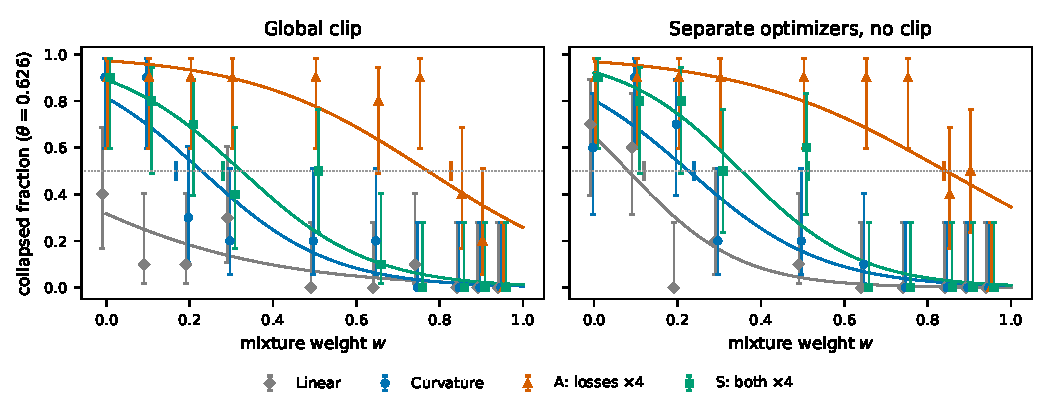
\includegraphics[width=\textwidth]{generated/v4/fig_e4_curves.pdf}
\caption{E4 (MAPPO on LBF): observed collapse proportions at $\theta=0.626$ with 95\% Wilson intervals (ten seeds per point; arms offset slightly in $w$), Firth fits (lines) and decreasing-isotonic crossings (vertical ticks at 0.5). The global-clip linear arm has no isotonic crossing in the grid and its Firth crossing lies below it (Table~\ref{tab:lbf}).}
\label{fig:lbf}
\Description{Two panels of collapse proportion against mixture weight for four arms; the loss-multiplier arm A stays collapsed to much higher w than the others in both panels.}
\end{figure}

\paragraph{Two pre-declared predictions are not confirmed.}
We had predicted that curvature would raise the LBF crossing under the global clip (P1) and that
separate optimizers would shrink the curvature and symmetric shifts (P3). Under the global clip the linear
arm's crossing lies below the sampled grid (Table~\ref{tab:lbf}), so P1 and the curvature half of P3 have
positive point estimates but are not identified; the symmetric half of P3 is not met. Both predictions
assumed the supply-chain clipping pathway, which LBF does not exhibit. The stored run labels used a
placeholder threshold of 0.5 instead of the declared 0.626; all E4 results here are recomputed at 0.626
from the stored team returns (deviation D4, Appendix~\ref{app:prereg}).

\begin{table}[t]
\caption{MAPPO on Level-Based Foraging (E4): crossings and paired contrasts. Ten seeds, ten mixture cells, 2M timesteps, 800 trajectories. $^{\dagger}$: point estimate outside the sampled grid (linear and curvature rarely collapse, so their crossings are not localized). $^{\ast}$: interval excludes zero.}
\label{tab:lbf}
\centering\scriptsize
\resizebox{\linewidth}{!}{%
\begin{tabular}{@{}lcccccc@{}}
\toprule
Optimizer & Linear & Curvature & A & S & A$-$S & A$-$linear \\
\midrule
Global clip & $-0.289$ $[-1.333,\,-0.001]$$^{\dagger}$ & $-0.370$ $[-2.288,\,0.009]$$^{\dagger}$ & $0.525$ $[0.188,\,0.719]$ & $0.107$ $[-0.065,\,0.225]$ & $+0.418$$^{\ast}$ $[+0.218,\,+0.553]$ & $+0.814$$^{\ast}$ $[+0.422,\,+1.725]$ \\
Separate, no clip & $0.003$ $[-0.179,\,0.068]$ & $0.077$ $[-0.087,\,0.196]$ & $0.557$ $[0.250,\,0.724]$ & $0.077$ $[-0.126,\,0.237]$ & $+0.479$$^{\ast}$ $[+0.289,\,+0.613]$ & $+0.554$$^{\ast}$ $[+0.310,\,+0.718]$ \\
\bottomrule
\end{tabular}
}
\end{table}


\begin{figure}[!htbp]
\centering
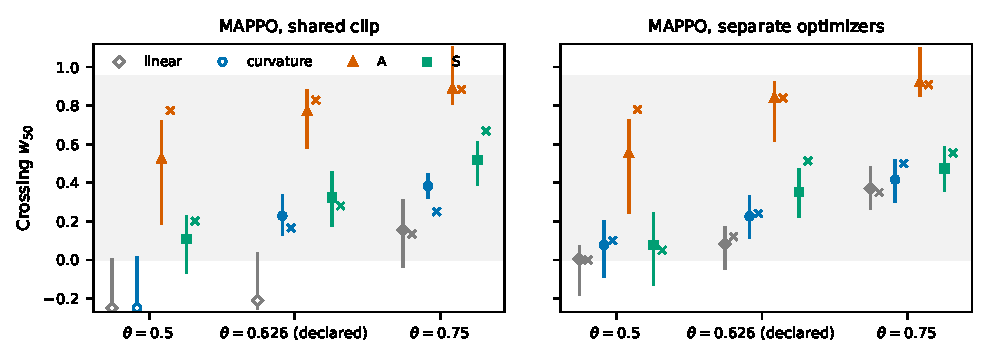
\includegraphics[width=\textwidth]{generated/v4/fig_lbf_sensitivity.pdf}
\caption{E4 estimator and label sensitivity. Firth crossings (markers, with 95\% seed-block intervals; open markers lie outside the sampled grid, which is shaded) and decreasing-isotonic crossings (crosses) for each arm, at the declared label threshold and two alternatives. Values outside $[-0.25,1.1]$ are drawn at the edge. The declared analysis is the middle group of each panel.}
\label{fig:lbf_sensitivity}
\Description{Two panels, one per optimizer mode, with three groups of four arms each; the loss-multiplier arm is highest in every group under both estimators.}
\end{figure}

% =======================================================================

\FloatBarrier

\section{Robustness and Sensitivity}
\label{sec:robustness}

\paragraph{A well-defined boundary exists at fixed training budget.}
At 300k steps on the supply-chain PPO substrate, collapse has a clear, tightly-estimated boundary in
reward-weighting space (Figure~\ref{fig:boundary}): the midpoint is \Headline{}. Observed
proportions and Wilson intervals show the sampled support of the crossing.

\paragraph{``Collapse'' is an operational threshold crossing, not a confirmed attractor.}
We tested the continuous base-stock statistic $\bar S$ for a distinct dynamical regime with bootstrap
95\% CIs on Sarle's bimodality coefficient~\citep{pfister2013bimodality} and Hartigan's dip
test~\citep{hartigan1985dip} in each cell of the legacy curvature-only sweep ($\lambda=1$,
$\alpha{=}\beta{=}0.88$; $w\in\{.5,.65,.75,.85,.95\}$; $n=20$ seeds per cell).
Sarle's coefficient rises near the crossing (0.59 at $w{=}0.65$ and 0.57 at $w{=}0.75$, both above the
0.555 rule of thumb) but its CI straddles the threshold everywhere, and the dip test never rejects
unimodality ($p\ge0.30$). At $n=20$ the dip test, calibrated against the uniform least-favorable null,
has little power, so non-rejection is not evidence of unimodality; it only means the data do not
establish a second regime. We therefore use \emph{threshold-defined behavioral crossing} throughout.

\begin{figure}[!htbp]
\centering
\includegraphics[width=.46\textwidth]{generated/boundary_observed.pdf}
\caption{Finite-budget supply PPO crossings in the legacy sweep. Top and middle: observed collapse proportions with 95\% Wilson intervals, Firth curves drawn only over sampled grids, midpoint lines and seed-block 95\% CI bands. Bottom: independently fitted horizons; budgets count requested agent transitions.}
\label{fig:boundary}
\Description{Observed collapse proportions and fitted curves at 150k and 300k, followed by the four estimated finite-budget midpoints and intervals.}
\end{figure}

\paragraph{The boundary is finite-horizon.}
In the legacy cross-sectional sweep the linear-reward boundary slides left with budget: 0.821, 0.666,
0.622 and 0.572 at 150k, 300k, 450k and 900k requested agent transitions
(Figure~\ref{fig:boundary}). These are separate finite-budget estimates and say nothing about
within-policy recovery.

\paragraph{Refined single-platform cohort (E3).}
To follow the same policies, we trained 270 trajectories to 3.6M transitions, evaluated every 150k: linear,
curvature-only and $\lambda=7$ rewards, ten seeds, and nine mixture cells
$\{.2,.4,.6,.65,.7,.75,.8,.85,1\}$. The four cells between .6 and .85 were added because a coarser
five-cell grid gave zero-width bootstrap intervals there. E3 uses the \emph{default} optimizer
configuration (single Adam step, global clip, raw rewards). Section~\ref{sec:optimizer} shows that in this
configuration reward scale alone moves the crossing, so the E3 contrasts below include that scale pathway:
they measure how transform effects evolve with budget under the default learner, not loss asymmetry. The
multiplier-minus-curvature difference is positive at every primary budget but shrinks, from
\VfourHorizonStart{} at 300k to \VfourHorizonEnd{} at 3.6M (Table~\ref{tab:horizon},
Figure~\ref{fig:horizon}). The $\lambda=7$ crossing falls monotonically,
whereas the linear and curvature-only crossings fall until 900k and then rise again. No condition meets
the pre-declared stability criterion, a 3.6M$-$1.8M interval within $\pm.05$
(Table~\ref{tab:horizon_stability}), so all readings are budget-conditional.

\paragraph{Collapse is not absorbing, and neither is non-collapse.}
Conditioning on the 300k label, many collapsed trajectories recover by 3.6M and some initially
non-collapsed ones relapse (Table~\ref{tab:horizon_stability}). The non-monotone linear and curvature
crossings reflect this relapse at high $w$. Cell-level counts are in Appendix~\ref{app:horizon}.

\begin{table}[t]
\caption{Refined single-platform horizon cohort (E3): nine mixture cells $\{.2,.4,.6,.65,.7,.75,.8,.85,1\}$, ten seeds, 270 trajectories trained to 3.6M and evaluated every 150k. Crossings with 95\% seed-block intervals; last row is the paired contrast.}
\label{tab:horizon}
\centering\scriptsize
\resizebox{\linewidth}{!}{%
\begin{tabular}{@{}lcccc@{}}
\toprule
Condition & 300k & 900k & 1.8M & 3.6M \\
\midrule
Linear & $0.663$ $[0.628,\,0.698]$ & $0.512$ $[0.449,\,0.584]$ & $0.535$ $[0.471,\,0.599]$ & $0.578$ $[0.515,\,0.643]$ \\
Curvature only & $0.587$ $[0.540,\,0.629]$ & $0.473$ $[0.400,\,0.558]$ & $0.523$ $[0.453,\,0.597]$ & $0.559$ $[0.513,\,0.612]$ \\
$\lambda=7$ & $0.877$ $[0.843,\,0.909]$ & $0.760$ $[0.745,\,0.775]$ & $0.710$ $[0.690,\,0.730]$ & $0.681$ $[0.634,\,0.713]$ \\
$\lambda7-$curvature & $+0.291$$^{\ast}$ $[+0.233,\,+0.341]$ & $+0.287$$^{\ast}$ $[+0.193,\,+0.364]$ & $+0.187$$^{\ast}$ $[+0.123,\,+0.247]$ & $+0.121$$^{\ast}$ $[+0.064,\,+0.177]$ \\
\bottomrule
\end{tabular}
}
\end{table}

\begin{table}[t]
\caption{Late-budget change and within-policy outcomes (E3). Stability requires the 3.6M$-$1.8M interval to lie within $\pm.05$ (pre-declared for v4). Recovery: collapsed at 300k, not collapsed at 3.6M; relapse: the reverse.}
\label{tab:horizon_stability}
\centering\small
\begin{tabular}{@{}lcccc@{}}
\toprule
Condition & 3.6M$-$1.8M & Stable & Recovered & Relapsed \\
\midrule
Linear & $+0.043$ $[-0.008,\,+0.095]$ & no & 14/39 & 8/51 \\
Curvature only & $+0.036$ $[-0.029,\,+0.105]$ & no & 4/28 & 4/62 \\
$\lambda=7$ & $-0.029$ $[-0.071,\,+0.001]$ & no & 34/76 & 0/14 \\
\bottomrule
\end{tabular}
\end{table}


\paragraph{Estimators, seeds and intervals.}
Logistic, probit and isotonic crossings agree within 0.018 on the supply chain
(Appendix~\ref{app:estimation}); on LBF they differ more, but not in the A$-$S ordering
(Figure~\ref{fig:lbf_sensitivity}). Leaving out any one of the ten training seeds changes the sign of none of
the principal contrasts (Table~\ref{tab:loso}). An independent 10,000-draw bootstrap reproduces every
principal interval to within \VrvMCShift{}, and a coverage-calibrated \VrvCalLevel{} interval changes none of
the \VrvNContrasts{} principal verdicts (Table~\ref{tab:results}). Stored labels are recomputed from the stored
evaluation statistics by one module that checks each threshold against the pre-registration text
(Appendix~\ref{app:artifact}).

% =======================================================================

\section{Limitations}
\label{sec:limitations}

\paragraph{Mechanism.} The shared-clip part of the symmetric shift is isolated by an intervention (E6). The
remainder is removed by reward normalization and, in an independent fresh-seed cohort, by a critic-only target
normalization (PopArt), which attributes it to critic target scale at the declared 95\% level. At the
coverage-calibrated level the fresh cohort's change includes zero, and it excludes zero only when both cohorts are
pooled. How much of Adam's partial compensation is due to the varying clip factor and how much to $\epsilon$ is not
isolated.

\paragraph{Reward moments.} A and S differ in the training reward's mean and variance as well as in the
gain-to-loss ratio. The online control matches A's training-reward mean and SD but not its shape, and its map is
nonstationary where A's is fixed; \VeightClamp{} of its \VeightNA{} runs reached the declared bound on the scale.
With a raw-target critic, the part of the asymmetric effect not explained by the first two moments is small
(\VeightAMonPlain{}), and a moment-matched symmetric reward reproduces most of the loss-only shift.

\paragraph{Statistics.} Ten training seeds per cell give contrast intervals of about $\pm0.1$ at 300k and up to
$\pm0.17$ at 3.6M, and the declared 95\% intervals under-cover at this sample size (Section~\ref{sec:stats}).
Intervals that include zero are reported as no detectable effect, and none would support equivalence at a
$\pm0.05$ margin. The 24-checkpoint E5 reading is exploratory and its intervals are pointwise.

\paragraph{Information structure and generality.} The supply-chain policy is a fully observed shared controller
without agent identity (Section~\ref{sec:method}); the results say nothing about decentralized information.
Two small environments and one PPO implementation (SB3 2.8.0) are tested; other implementations, clipping
conventions and value normalizations may couple actor and critic differently, and LBF does not exhibit the
supply-chain clipping pathway. In LBF the linear arm's crossing under the global clip lies below the sampled
grid, so contrasts with it are not identified. No condition has a stable crossing by 3.6M, so all readings are
finite-budget. An earlier ablation on the supply chain found no interior crossing for PPO, QMIX or IQL on a
coarse 11-level discretization of the base-stock action. Crossings are conditional on the behavioral label and
the sampled grid; non-bracketed estimates are reported, not clipped.

\paragraph{Pre-registration record.} E4's stored labels used a fallback threshold of 0.5 instead of the
declared 0.626 because a calibration file was missing from the frozen source; all E4 results are recomputed
from the stored team returns (deviation D4). Each stored team return equals the mean of the run's ten stored
per-episode returns (largest difference $\VdaEMaxDiff{}$, all 800 runs), and the stored labels are exactly the
0.5-threshold labels. \VdaETies{} run has a return of exactly 0.75, so its label in the $\theta=0.75$ sensitivity
analysis depends on floating-point summation order; no other threshold is affected. The provenance of 0.626 is an earlier calibration whose raw
records are not archived, so the threshold itself is taken as declared, not re-derived; Figure~\ref{fig:lbf_sensitivity}
shows that the A$-$S ordering does not depend on it.

% =======================================================================

\section{Discussion and Conclusion}
\label{sec:discussion}

\paragraph{What is established.}
Three findings are supported at the level of evidence stated in Table~\ref{tab:hierarchy} and
Sections~\ref{sec:asymmetric} and~\ref{sec:lbf}. First, a finite-budget crossing along the reward-weighting
dial can be estimated with seed-paired intervals of roughly $\pm0.03$--$0.1$, but it moves with training
budget, does not stabilize by 3.6M transitions, and depends on the optimizer configuration. Second, under
SB3's default PPO a symmetric reward multiplier moves the crossing at least as far as a loss-only multiplier,
and the shared gradient clip is the identified pathway for part of it: the critic takes the clip, the
actor's parameter update shrinks, and clipping the two separately restores the update and reduces the shift.
Third, with separate optimizers and
normalized rewards, a loss-only multiplier moves the crossing relative to a symmetric control on the
supply chain, through 3.6M transitions, and an asymmetric transform moves it on Level-Based Foraging by a
different route. Against a symmetric control matched online in mean and SD (E8), the supply-chain effect is
large when the critic's targets are normalized and small, though detectable, when they are not. None of this is evidence about loss aversion as a psychological mechanism: the effect is
a property of the transformed training signal, and in LBF it is plainly an incentive change on a costly
cooperative action.

\paragraph{Implications for reward-transform experiments.}
The practical lesson is about design, not about loss asymmetry. A reward-transform comparison in
actor--critic MARL should include a symmetric-scaling control at the same multiplier and should report
whether actor and critic share a gradient clip and whether rewards or value targets are normalized; without
these, a change in reward scale can pass for a change in reward shape.

\paragraph{Implications for actor--critic optimization.}
The confound needs two ingredients that are SB3 PPO's defaults: an unnormalized critic and one gradient
clip over actor and critic. Advantages are normalized per minibatch, so the actor's loss is nearly
scale-free, but the critic's gradient grows with the reward and takes the clip budget. Cooperative PPO
implementations that normalize value targets by default~\citep{yu2022surprising} should be less exposed;
we did not test them.

\paragraph{Interpreting finite-budget crossings.}
$\wcrit$ is a 50\% point of a fitted response curve at a stated budget, learner, reward unit and label. It is
not a critical point, a safe operating point or an asymptotic property. Trajectories both recover from
and relapse into collapse (Table~\ref{tab:horizon_stability}), so the crossing summarizes a population of
training outcomes, not an attractor. Contrasts between arms within one configuration are more stable than
absolute crossings: in E5 the absolute crossings fall and rise again, while A$-$S stays positive. A
deployment requirement such as at most 5\% collapse would need its own probability target and uncertainty
assessment.

\paragraph{Reproducibility.}
All E1--E8 runs share one platform; trained policies are not bit-reproducible across hardware and software
builds, but labels agree in \VfourAgreeControl{} of matched runs, so we claim reproducibility of labels and
crossings, not of policies. The artifact rebuilds every reported table, figure and number from per-run
records with one command (Appendix~\ref{app:artifact}).

\paragraph{Conclusion.}
Reward centralization is usually treated as a direction: more team signal helps. It also has a measurable
finite-budget location, $\wcrit$, that moves with reward transforms, training budget and the optimizer.
Measured with default SB3 PPO, a symmetric reward multiplier and a loss-only multiplier cannot be told
apart, because a shared gradient clip lets reward scale reach the actor's updates. With that coupling
removed and rewards normalized, the loss-only multiplier moves the crossing and the symmetric one produces
no detectable shift, in the tested configurations of two environments. How much of that shift is about sign
asymmetry rather than the reward's moments depends on the critic. With raw value targets, a symmetric control with
matched mean and SD reproduces most of it, leaving a small asymmetric remainder; with normalized value targets it
reproduces almost none. Reward-transform comparisons in
actor--critic MARL should therefore include symmetric-scaling controls and report the optimizer coupling,
gradient clipping, reward or value normalization and training budget under which they were run.

% =======================================================================
\section*{Ethical Statement}

This work is entirely simulated, with no human subjects or personal data. Reported thresholds are
substrate-specific and must be re-measured before use.


\bibliographystyle{tmlr}
\bibliography{references}

\clearpage
\appendix
\suppressfloats[t]
\section{Experimental Configuration}
\label{app:configuration}

\paragraph{Supply-chain environment and learner.}
The six-node \texttt{NetworkManagement-v1} network has 30-period episodes. Node 1 is scripted to order
20 units per period, split equally across its action entries; nodes 2--6 are controlled by one
parameter-shared PPO policy. Every trainable node's lane receives the same full or-gym observation of the
network state, with no agent identifier; actions are padded to the largest per-node action dimension, and each
node uses its leading entries, so under deterministic evaluation all five nodes receive the same action
vector. PPO uses Stable-Baselines3 2.8.0 with \texttt{n\_steps} $=128$, minibatch size 256, ten
optimization epochs, learning rate $3\times10^{-4}$, discount $0.99$, GAE coefficient $0.95$, policy
clip $0.2$, value-loss coefficient $0.5$, zero entropy coefficient, normalized minibatch advantages,
separate actor and critic MLPs of width 64, one Adam optimizer with SB3's implicit $\epsilon=10^{-5}$,
and global gradient max-norm $0.5$. Training is CPU-only and single-threaded, with an explicit simulator
random stream per environment.

\paragraph{Budget arithmetic.}
Budgets count requested agent transitions. Five lanes and 128-step rollouts add 640 transitions per
rollout, and training stops at the first completed rollout at or beyond the request: 300k requested
transitions execute 300,160 (469 rollouts), and each 150k checkpoint is evaluated at the first rollout
boundary after it. One agent transition is one node's step, so 300,160 transitions are 60,032 joint
environment periods (about 2,001 episodes).

\paragraph{Reward, reference point and controls.}
Each agent receives $x_i(w)=(1-w)r_i^{\mathrm{local}}+wr^{\mathrm{global}}$ before any transform. The
linear condition uses $v(x)=x$; curvature-only uses $\phi(x)=\operatorname{sign}(x)|x|^{.88}$; the
loss-multiplier condition uses $v_\lambda(x)=\phi(x)$ for $x\ge0$ and $\lambda\phi(x)$ for $x<0$. E1 and
E2 use the reference $z_0=-2.6281398333$, fixed before any of their runs as the pooled mean of raw
blended rewards from 40 untreated curvature-only calibration policies, with 7,500 samples at each of
the eight E1 mixture cells (60,000 samples). With $u=x-z_0$ and
$s_{\mathrm{in}}=1$, the arms are B$=\phi(u)$ ($s_{\mathrm{out}}=1$), A$=v_7(u)$ ($s_{\mathrm{out}}=1$),
S$=7\phi(u)$ ($s_{\mathrm{out}}=1/7$) and R$=3.451\,\phi(u)$ ($s_{\mathrm{out}}=1/3.451$, where 3.451 is
A's pooled transformed-reward RMS divided by B's in the earlier direct control). E3 uses reference zero.

\paragraph{Optimizer interventions.}
\texttt{separate\_no\_clip} builds two Adam optimizers with the default settings, one over the actor
parameters (policy MLP, action head, log-standard-deviation) and one over the critic parameters (value
MLP and head), applies the unchanged PPO loss, and skips gradient clipping; execution aborts if any
trainable parameter is shared. \texttt{VecNormalize} divides rewards by the running standard deviation of
discounted returns ($\gamma=0.99$, $\epsilon=10^{-8}$, reward clip 10, no observation normalization). E2
passes \texttt{optimizer\_kwargs=\{eps: 1e-8\}}. E6's \texttt{groupwise\_clip} keeps one Adam optimizer and
clips the actor and critic gradients to norm 0.5 separately; E6 also records, at every optimizer step and
for each parameter group, the post-clip gradient norm and the norm of the parameter change, by copying the
parameters before the step. Every run logs per-minibatch actor, critic and total
gradient norms before and after the clipping step.

\paragraph{Labels.}
The supply-chain label is $\mathbf{1}[\bar S<10\wedge\bar\pi\le-127.1]$, with $\bar S$ the mean over
nodes 2--6 of the deterministic base-stock target $250(a_1+1)$ at the reset of evaluation seed $10s$,
and $\bar\pi$ the ten-episode mean total profit on seeds $10s,\ldots,10s+9$. The LBF label is native
team return below 0.626 over ten deterministic episodes on seeds $10s,\ldots,10s+9$; the native return
excludes the effort cost.

\paragraph{LBF learner.}
MAPPO uses SB3 PPO with a centralized-critic policy: the actor's features come from the agent's own
observation and the critic's from the concatenated global state (feature width 128; actor heads
$[64,64]$, critic heads $[128,128]$), eight parallel environment copies, \texttt{n\_steps} $=256$,
minibatch 512, entropy coefficient 0.01, and \texttt{lbforaging} 2.0.0. In a check at 100k timesteps
on one cell and seed, the global-clip runner reproduced the legacy LBF runner's team return exactly.

\section{Boundary Estimation and Diagnostics}
\label{app:estimation}

For each fixed configuration we fit $P(Y=1\mid w)=\sigma(b_0+b_1w)$ by Firth logistic regression and
report $w_{50}=-b_0/b_1$. A point estimate is reported only with an identified nonzero slope; observed
proportions are inspected separately for adjacent cells bracketing $.5$. Confidence intervals use 2,000
percentile-bootstrap draws of complete training-seed blocks (multinomial weights over the ten seeds;
random seed 20261015 for E1--E8; E8's fresh-seed cohort uses the same weights over seeds 52--61). The same weight vector is used for every condition in an experiment,
so differences are seed-paired. Fits outside the grid and non-converged draws are retained and counted.
Intervals are pointwise; no simultaneous statement across checkpoints or cells is made.

\paragraph{Interval coverage and bootstrap stability.}
These checks were added in revision; they are not pre-registered and change no reported estimate
(\texttt{analysis/stat\_checks.py}). First, each principal contrast is re-derived from the per-run tables and
asserted equal to the stored result. Second, an independent set of 10,000 draws (seed 20261105) moves no interval
endpoint by more than \VrvMCShift{}. Third, Table~\ref{tab:coverage} simulates the design from two logistic
curves, steep ($b_1=-20$) and shallow ($b_1=-8$), as found in the E1 and E7 fits, with a null contrast or a
contrast of the size observed, with and without a per-seed logit intercept (SD 1) shared by both arms. The
percentile intervals under-cover at ten seeds, as percentile bootstraps do at small sample sizes; nominal
\VrvCalLevel{} intervals reach at least \VrvCalCovMin{}. Table~\ref{tab:results} reports both levels.

\begin{table}[H]
\caption{Simulated behaviour of the seed-block percentile intervals at the paper's design: ten seeds, the E1 grid, one label per seed and cell, 1,000 replicates per row, 2,000 bootstrap draws. Each scenario has two arms; ``seed SD'' is the standard deviation of a per-seed logit intercept shared by both arms. Coverage is of the true crossing ($w_{50}$) and of the true paired contrast; the last block is the fraction of replicates whose contrast interval excludes zero, which is the false-positive rate under a null contrast and power otherwise.}
\label{tab:coverage}
\centering\scriptsize\setlength{\tabcolsep}{3pt}
\begin{tabular}{@{}lcccccccccccc@{}}
\toprule
& & & & \multicolumn{3}{c}{Coverage of $w_{50}$} & \multicolumn{3}{c}{Coverage of contrast} & \multicolumn{3}{c}{Interval excludes 0} \\
\cmidrule(lr){5-7}\cmidrule(lr){8-10}\cmidrule(l){11-13}
Scenario & Seed SD & True $w_{50}$ & True contrast & 95 & 97.5 & 99 & 95 & 97.5 & 99 & 95 & 97.5 & 99 \\
\midrule
steep, null & 0 & $0.400$ & $+0.00$ & 0.923 & 0.942 & 0.963 & 0.913 & 0.940 & 0.955 & 0.087 & 0.060 & 0.045 \\
steep, null & 1 & $0.400$ & $+0.00$ & 0.917 & 0.944 & 0.971 & 0.904 & 0.925 & 0.948 & 0.096 & 0.075 & 0.052 \\
steep, +0.10 & 0 & $0.400$ & $+0.10$ & 0.919 & 0.944 & 0.966 & 0.899 & 0.938 & 0.961 & 0.822 & 0.759 & 0.670 \\
steep, +0.10 & 1 & $0.400$ & $+0.10$ & 0.922 & 0.947 & 0.966 & 0.911 & 0.941 & 0.961 & 0.806 & 0.751 & 0.659 \\
shallow, null & 0 & $0.438$ & $+0.00$ & 0.890 & 0.931 & 0.950 & 0.905 & 0.937 & 0.962 & 0.095 & 0.063 & 0.038 \\
shallow, null & 1 & $0.438$ & $+0.00$ & 0.889 & 0.929 & 0.962 & 0.912 & 0.940 & 0.961 & 0.088 & 0.060 & 0.039 \\
shallow, +0.20 & 0 & $0.438$ & $+0.20$ & 0.884 & 0.915 & 0.939 & 0.900 & 0.927 & 0.947 & 0.944 & 0.909 & 0.849 \\
shallow, +0.20 & 1 & $0.438$ & $+0.20$ & 0.912 & 0.937 & 0.960 & 0.904 & 0.936 & 0.961 & 0.934 & 0.898 & 0.841 \\
\bottomrule
\end{tabular}
\end{table}


Logistic, probit and decreasing isotonic fits are sensitivity estimators on the same rows. The isotonic
fit is weighted pool-adjacent-violators; its crossing is linear interpolation between the last cell with
fitted probability at least $.5$ and the first below it, and a plateau at exactly $.5$ is reported as an
interval with its midpoint used for comparison. The maximum spread among the three point estimators on
the legacy supply-chain sweep is 0.018. Table~\ref{tab:isotonic} compares Firth and isotonic crossings for
every in-grid E1--E4 fit.

\begin{table}[H]
\caption{Agreement between Firth and decreasing-isotonic crossings for every in-grid fit. LBF collapse proportions are far from the logistic shape for some arms, which is why E4 shows the largest gaps; E4's A$-$S conclusion holds under both estimators (Table~\ref{tab:lbf_theta}).}
\label{tab:isotonic}
\centering\small
\begin{tabular}{@{}lrr@{}}
\toprule
Experiment & Max $|$Firth$-$isotonic$|$ & Median \\
\midrule
E1/E2 (20 fits) & 0.055 & 0.019 \\
E3 (72 fits) & 0.047 & 0.016 \\
E4, $\theta=0.626$ (7 in-grid fits) & 0.161 & 0.044 \\
\bottomrule
\end{tabular}
\end{table}

\begin{table}[H]
\caption{Leave-one-seed-out sensitivity of the principal contrasts (exploratory). Each contrast is refitted ten times on nine training seeds; the range of the ten point estimates and the number that keep the full-data sign are shown. E4 uses the pre-declared $\theta=0.626$.}
\label{tab:loso}
\centering\small
\begin{tabular}{@{}llrcr@{}}
\toprule
Experiment & Contrast & All seeds & Leave-one-out range & Same sign \\
\midrule
E1 default & S$-$B & $+0.357$ & $[+0.325,\,+0.384]$ & 10/10 \\
E1 default & A$-$S & $-0.074$ & $[-0.098,\,-0.048]$ & 10/10 \\
E1 decoupled & S$-$B & $-0.049$ & $[-0.072,\,-0.031]$ & 10/10 \\
E1 decoupled & A$-$S & $+0.237$ & $[+0.200,\,+0.267]$ & 10/10 \\
E5, 3.6M & S$-$B & $-0.049$ & $[-0.102,\,-0.013]$ & 10/10 \\
E5, 3.6M & A$-$S & $+0.154$ & $[+0.134,\,+0.189]$ & 10/10 \\
E6 per-group clip & S$-$B & $+0.150$ & $[+0.135,\,+0.169]$ & 10/10 \\
E6 per-group clip & A$-$S & $+0.168$ & $[+0.148,\,+0.193]$ & 10/10 \\
E4 global clip & A$-$S & $+0.447$ & $[+0.423,\,+0.504]$ & 10/10 \\
E4 separate & A$-$S & $+0.490$ & $[+0.453,\,+0.533]$ & 10/10 \\
\bottomrule
\end{tabular}
\end{table}

\FloatBarrier
\input{generated/supply_cells}
\input{generated/lambda_table}
\FloatBarrier

\section{Pre-registration and Deviations}
\label{app:prereg}

E1--E4 were declared in a pre-registration written before any of their outcomes existed; E5--E8 were
declared later, in response to reviews of an earlier draft, again before any of their runs. Each of E5--E8
had a pre-launch gate that reproduced a completed earlier run bit-for-bit (an E1 run; for E8, an E7 run) through the new code path. Source,
design and protocol hashes were frozen before E1 launched, and the E4 runner's hash before E4 launched,
after a timing check. Launch scripts refused to run on any hash mismatch. The record shows four
departures, none changing a design:
(i)~the frozen E1 runner omitted a protocol field read at evaluation, so every run crashed after training
and before producing a label; the field was added with the mapping used by the earlier direct control,
before any outcome existed;
(ii--iii)~two analysis-code errors (floating-point grid keys; the condition name ``null'' read as missing)
raised exceptions before any fit was computed;
(iv)~found after the E4 analysis: the LBF label function reads its threshold from a calibration file that was
absent from the frozen source and silently fell back to a placeholder of 0.5, so the stored E4 labels use
$\theta=0.5$ rather than the declared 0.626. Because every run stores its team return, all E4 results are
recomputed at $\theta=0.626$; the 0.5 analysis is kept as a sensitivity result (Table~\ref{tab:lbf_theta}).
The pre-declared predictions that failed are reported in the main text: the Adam-$\epsilon$ route (E2)
two of three LBF predictions (E4), and in E7 the critic-target attribution (inconclusive), the moment
control under the plain critic and the moment-matching check. An equality gate run before E1 reproduced the earlier platform's
labels in 8/8 cells, but not its policies bit-for-bit, so archived runs were not reused.

\section{Refined Horizon Cohort}
\label{app:horizon}

\begin{table}[t]
\caption{E3 observed collapsed trajectories out of ten seeds per mixture cell at the four primary budgets. Full checkpoint records are in the archive.}
\label{tab:horizon_cells}
\centering\scriptsize
\begin{tabular}{@{}llrrrrrrrrr@{}}
\toprule
Condition & Budget & $w{=}0.2$ & $w{=}0.4$ & $w{=}0.6$ & $w{=}0.65$ & $w{=}0.7$ & $w{=}0.75$ & $w{=}0.8$ & $w{=}0.85$ & $w{=}1$ \\
\midrule
Linear & 300k & 10 & 10 & 8 & 6 & 2 & 2 & 1 & 0 & 0 \\
 & 900k & 10 & 9 & 1 & 2 & 0 & 0 & 0 & 0 & 0 \\
 & 1.8M & 10 & 9 & 2 & 2 & 1 & 1 & 0 & 0 & 0 \\
 & 3.6M & 10 & 9 & 3 & 3 & 2 & 1 & 4 & 1 & 0 \\
Curvature only & 300k & 10 & 10 & 6 & 1 & 0 & 0 & 0 & 1 & 0 \\
 & 900k & 10 & 7 & 2 & 1 & 0 & 0 & 0 & 0 & 0 \\
 & 1.8M & 10 & 8 & 3 & 3 & 0 & 0 & 0 & 0 & 0 \\
 & 3.6M & 10 & 10 & 3 & 3 & 0 & 0 & 1 & 0 & 1 \\
$\lambda=7$ & 300k & 10 & 10 & 10 & 10 & 10 & 10 & 9 & 7 & 0 \\
 & 900k & 10 & 10 & 10 & 10 & 10 & 7 & 0 & 0 & 0 \\
 & 1.8M & 10 & 10 & 10 & 9 & 7 & 1 & 0 & 0 & 0 \\
 & 3.6M & 10 & 10 & 8 & 6 & 6 & 1 & 1 & 0 & 0 \\
\bottomrule
\end{tabular}
\end{table}


\begin{figure}[H]
\centering
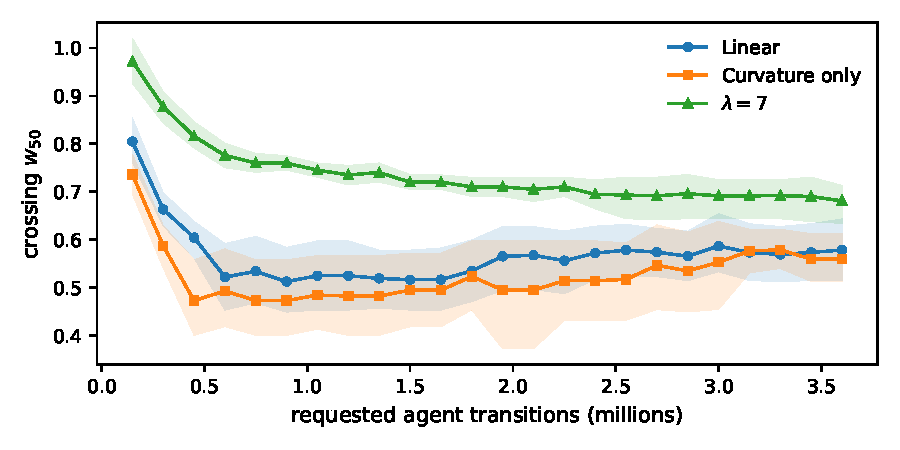
\includegraphics[width=.78\textwidth]{generated/v4/horizon_curves.pdf}
\caption{E3 crossings at every checkpoint (lines) with pointwise 95\% seed-block bands. Default optimizer; nine mixture cells, ten seeds per cell and condition.}
\label{fig:horizon}
\Description{Three crossing curves over training budget: lambda seven decreasing throughout; linear and curvature-only falling to 900k and rising afterwards.}
\end{figure}
\FloatBarrier

\section{Optimizer Factorial Details}
\label{app:factorial}

\begin{table}[H]
\caption{Change in each contrast relative to the default cell (global clip, raw reward), paired by seed. $^{\ast}$: interval excludes zero.}
\label{tab:factorial_interactions}
\centering\footnotesize
\begin{tabular}{@{}lcccc@{}}
\toprule
Intervention & $\Delta$(A$-$S) & $\Delta$(A$-$B) & $\Delta$(S$-$B) & $\Delta$(R$-$B) \\
\midrule
Global clip, normalized reward & \begin{tabular}[t]{@{}c@{}}$+0.311$$^{\ast}$\\[-1pt]{\scriptsize $[+0.220,\,+0.402]$}\end{tabular} & \begin{tabular}[t]{@{}c@{}}$+0.003$\\[-1pt]{\scriptsize $[-0.130,\,+0.146]$}\end{tabular} & \begin{tabular}[t]{@{}c@{}}$-0.308$$^{\ast}$\\[-1pt]{\scriptsize $[-0.443,\,-0.158]$}\end{tabular} & \begin{tabular}[t]{@{}c@{}}$-0.195$$^{\ast}$\\[-1pt]{\scriptsize $[-0.349,\,-0.046]$}\end{tabular} \\
Separate optimizers, raw & \begin{tabular}[t]{@{}c@{}}$+0.248$$^{\ast}$\\[-1pt]{\scriptsize $[+0.136,\,+0.373]$}\end{tabular} & \begin{tabular}[t]{@{}c@{}}$+0.051$\\[-1pt]{\scriptsize $[-0.071,\,+0.161]$}\end{tabular} & \begin{tabular}[t]{@{}c@{}}$-0.197$$^{\ast}$\\[-1pt]{\scriptsize $[-0.366,\,-0.021]$}\end{tabular} & \begin{tabular}[t]{@{}c@{}}$-0.229$$^{\ast}$\\[-1pt]{\scriptsize $[-0.350,\,-0.104]$}\end{tabular} \\
Separate optimizers, normalized & \begin{tabular}[t]{@{}c@{}}$+0.311$$^{\ast}$\\[-1pt]{\scriptsize $[+0.209,\,+0.396]$}\end{tabular} & \begin{tabular}[t]{@{}c@{}}$-0.096$\\[-1pt]{\scriptsize $[-0.239,\,+0.034]$}\end{tabular} & \begin{tabular}[t]{@{}c@{}}$-0.407$$^{\ast}$\\[-1pt]{\scriptsize $[-0.565,\,-0.258]$}\end{tabular} & \begin{tabular}[t]{@{}c@{}}$-0.320$$^{\ast}$\\[-1pt]{\scriptsize $[-0.480,\,-0.174]$}\end{tabular} \\
Global clip, raw, Adam $\epsilon{=}10^{-8}$ & \begin{tabular}[t]{@{}c@{}}$+0.122$$^{\ast}$\\[-1pt]{\scriptsize $[+0.008,\,+0.253]$}\end{tabular} & \begin{tabular}[t]{@{}c@{}}$+0.023$\\[-1pt]{\scriptsize $[-0.087,\,+0.132]$}\end{tabular} & \begin{tabular}[t]{@{}c@{}}$-0.099$\\[-1pt]{\scriptsize $[-0.243,\,+0.033]$}\end{tabular} & \begin{tabular}[t]{@{}c@{}}$-0.090$\\[-1pt]{\scriptsize $[-0.201,\,+0.036]$}\end{tabular} \\
\bottomrule
\end{tabular}
\end{table}

\begin{table}[t]
\caption{Optimizer diagnostics (means over runs of per-minibatch means). Pre-clip critic and actor gradient norms, post-clip (applied) actor norm, actor share of squared gradient norm, fraction of minibatches whose norm exceeds 0.5, and transformed-reward RMS. With separate optimizers no clipping is applied, so the applied actor norm equals the pre-clip norm.}
\label{tab:factorial_diagnostics}
\centering\scriptsize
\resizebox{\linewidth}{!}{%
\begin{tabular}{@{}llrrrrrr@{}}
\toprule
Cell & Arm & Critic & Actor & Applied actor & Actor share & Over 0.5 & Reward RMS \\
\midrule
Global clip, raw (default) & B & 1,326.81 & 2.07 & 0.0015 & 0.000 & 1.000 & 8.7 \\
 & A & 3,425.24 & 1.83 & 0.0009 & 0.000 & 1.000 & 30.1 \\
 & S & 11,964.76 & 1.46 & 0.0002 & 0.000 & 1.000 & 56.9 \\
Global clip, normalized reward & B & 0.12 & 4.39 & 0.4967 & 0.989 & 0.999 & 9.9 \\
 & A & 0.14 & 4.22 & 0.4962 & 0.988 & 0.999 & 31.4 \\
 & S & 0.12 & 4.25 & 0.4966 & 0.989 & 0.999 & 68.9 \\
Separate optimizers, raw & B & 1,285.95 & 4.06 & 4.0562 & 0.000 & 1.000 & 9.8 \\
 & A & 3,737.64 & 3.63 & 3.6322 & 0.000 & 1.000 & 30.6 \\
 & S & 13,923.98 & 4.41 & 4.4090 & 0.000 & 1.000 & 64.1 \\
Separate optimizers, normalized & B & 0.12 & 3.86 & 3.8594 & 0.986 & 0.999 & 9.8 \\
 & A & 0.14 & 3.86 & 3.8567 & 0.985 & 0.999 & 31.5 \\
 & S & 0.12 & 3.99 & 3.9904 & 0.987 & 0.999 & 69.5 \\
Global clip, raw, Adam $\epsilon{=}10^{-8}$ & B & 1,286.02 & 2.70 & 0.0019 & 0.000 & 1.000 & 9.0 \\
 & A & 3,828.34 & 2.43 & 0.0011 & 0.000 & 1.000 & 31.1 \\
 & S & 11,698.56 & 2.42 & 0.0003 & 0.000 & 1.000 & 59.5 \\
\bottomrule
\end{tabular}
}
\end{table}

\begin{table}[H]
\caption{E1/E2 observed collapsed runs out of ten seeds per mixture cell at 300k.}
\label{tab:factorial_cells}
\centering\scriptsize
\begin{tabular}{@{}llrrrrrrrr@{}}
\toprule
Cell & Arm & $w{=}0$ & $w{=}0.2$ & $w{=}0.4$ & $w{=}0.5$ & $w{=}0.6$ & $w{=}0.7$ & $w{=}0.85$ & $w{=}1$ \\
\midrule
Global clip, raw (default) & B & 10 & 10 & 9 & 5 & 4 & 1 & 0 & 0 \\
 & A & 10 & 10 & 10 & 10 & 10 & 10 & 3 & 0 \\
 & S & 10 & 10 & 10 & 10 & 10 & 10 & 7 & 1 \\
 & R & 10 & 10 & 10 & 10 & 10 & 10 & 1 & 0 \\
Global clip, normalized reward & B & 10 & 6 & 4 & 2 & 0 & 0 & 0 & 0 \\
 & A & 10 & 10 & 9 & 8 & 4 & 3 & 0 & 0 \\
 & S & 10 & 8 & 4 & 2 & 1 & 0 & 0 & 0 \\
 & R & 10 & 10 & 3 & 1 & 0 & 0 & 0 & 0 \\
Separate optimizers, raw & B & 10 & 9 & 2 & 1 & 0 & 0 & 0 & 0 \\
 & A & 10 & 10 & 10 & 10 & 9 & 2 & 0 & 0 \\
 & S & 10 & 10 & 7 & 3 & 4 & 0 & 1 & 0 \\
 & R & 10 & 9 & 3 & 2 & 0 & 0 & 0 & 0 \\
Separate optimizers, normalized & B & 10 & 10 & 5 & 2 & 1 & 0 & 1 & 0 \\
 & A & 10 & 10 & 10 & 9 & 4 & 2 & 0 & 0 \\
 & S & 10 & 8 & 6 & 1 & 0 & 0 & 0 & 0 \\
 & R & 10 & 8 & 5 & 1 & 0 & 0 & 0 & 0 \\
Global clip, raw, Adam $\epsilon{=}10^{-8}$ & B & 10 & 10 & 5 & 4 & 1 & 2 & 0 & 0 \\
 & A & 10 & 10 & 10 & 10 & 10 & 9 & 0 & 0 \\
 & S & 10 & 10 & 10 & 9 & 9 & 4 & 2 & 0 \\
 & R & 10 & 10 & 10 & 6 & 7 & 3 & 0 & 0 \\
\bottomrule
\end{tabular}
\end{table}

\begin{table}[H]
\caption{Fraction of training rewards on the loss branch ($x-z_0<0$, $z_0=-2.628$), by mixture weight, for the default and the fully decoupled E1 cells. The fraction depends on $w$ and on the learned policy; near the crossings both branches are active.}
\label{tab:loss_occupancy}
\centering\scriptsize
\begin{tabular}{@{}llrrrrrrrr@{}}
\toprule
Cell & Arm & $w{=}0$ & $w{=}0.2$ & $w{=}0.4$ & $w{=}0.5$ & $w{=}0.6$ & $w{=}0.7$ & $w{=}0.85$ & $w{=}1$ \\
\midrule
Global clip, raw (default) & B & 0.59 & 0.63 & 0.50 & 0.37 & 0.26 & 0.18 & 0.10 & 0.08 \\
 & A & 0.59 & 0.65 & 0.58 & 0.57 & 0.55 & 0.49 & 0.13 & 0.07 \\
 & S & 0.59 & 0.64 & 0.57 & 0.54 & 0.48 & 0.37 & 0.17 & 0.08 \\
Separate optimizers, normalized & B & 0.58 & 0.58 & 0.32 & 0.18 & 0.14 & 0.10 & 0.08 & 0.07 \\
 & A & 0.58 & 0.62 & 0.51 & 0.38 & 0.24 & 0.17 & 0.09 & 0.08 \\
 & S & 0.58 & 0.52 & 0.24 & 0.19 & 0.14 & 0.11 & 0.09 & 0.07 \\
\bottomrule
\end{tabular}
\end{table}


\begin{figure}[H]
\centering
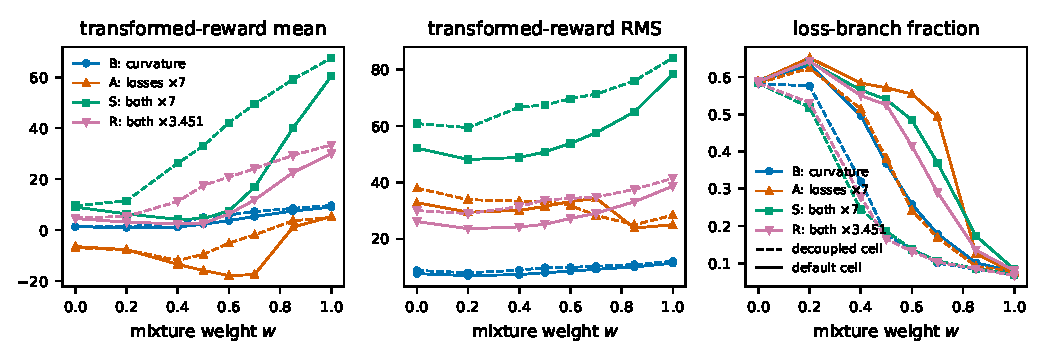
\includegraphics[width=\textwidth]{generated/v4/fig_reward_moments.pdf}
\caption{Transformed-reward moments over training in E1, by arm and mixture weight: mean, RMS and fraction on the loss branch (per-run means, averaged over seeds), for the default cell (solid) and the fully decoupled cell (dashed). The per-run tables keep these moments; per-rollout quantiles were also logged and are summarized for E7 in Table~\ref{tab:dist}.}
\label{fig:reward_moments}
\Description{Three line panels against mixture weight; A has a negative mean while S and R have growing positive means; RMS is largest for S.}
\end{figure}

\begin{figure}[H]
\centering
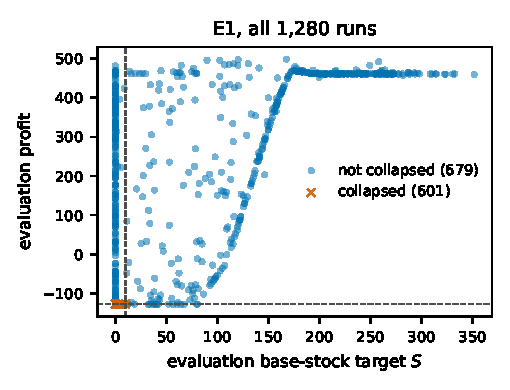
\includegraphics[width=.5\textwidth]{generated/v4/fig_label.pdf}
\caption{Collapse-label validation on all E1 runs: evaluation base-stock target $\bar S$ against evaluation profit, with the two label thresholds ($\bar S<10$, profit $\le-127.1$) dashed. Collapsed runs sit at the lazy-policy corner.}
\label{fig:label}
\Description{Scatter of profit against base-stock target; collapsed runs cluster at near-zero target and profit near minus 128.}
\end{figure}
\FloatBarrier

\begin{table}[H]
\caption{E7 training-reward and critic-target distributions. Per-rollout statistics of the transformed training reward (pooled over the five nodes) and of the rollout-buffer returns that the critic regresses, averaged over the 469 rollouts of each run and then over the 80 runs of each arm (ten seeds, eight cells). Quantile skewness is $(p_{90}+p_{10}-2p_{50})/(p_{90}-p_{10})$. M's reward statistics are reconstructed exactly from the logged B reward and M's frozen affine map; its fraction of negative rewards is not recoverable from the logs. Descriptive; not pre-registered.}
\label{tab:dist}
\centering\scriptsize\setlength{\tabcolsep}{4pt}
\begin{tabular}{@{}llrrrrrrrrr@{}}
\toprule
& & \multicolumn{7}{c}{Training reward (per rollout)} & \multicolumn{2}{c}{Critic targets} \\
\cmidrule(lr){3-9}\cmidrule(l){10-11}
Critic & Arm & Mean & SD & $p_{10}$ & $p_{50}$ & $p_{90}$ & Q-skew & Frac.\ $<0$ & Mean & SD \\
\midrule
Plain & B (curvature) & $+5.5$ & 7.0 & $-1.0$ & $+5.8$ & $+13.0$ & $+0.01$ & 0.23 & $+68$ & 50 \\
Plain & A (losses $\times7$) & $-6.6$ & 22.4 & $-25.7$ & $-3.9$ & $+12.2$ & $-0.12$ & 0.40 & $-104$ & 113 \\
Plain & S (both $\times7$) & $+31.5$ & 47.5 & $-15.1$ & $+31.0$ & $+88.9$ & $+0.10$ & 0.30 & $+256$ & 270 \\
Plain & M (affine of B) & $-13.5$ & 26.2 & $-38.9$ & $-15.4$ & $+20.0$ & $+0.18$ & -- & $-185$ & 148 \\
PopArt & B (curvature) & $+5.5$ & 7.0 & $-1.2$ & $+5.9$ & $+13.0$ & $-0.01$ & 0.23 & $+73$ & 53 \\
PopArt & A (losses $\times7$) & $-3.1$ & 22.2 & $-21.0$ & $+1.5$ & $+12.6$ & $-0.27$ & 0.32 & $-70$ & 123 \\
PopArt & S (both $\times7$) & $+38.5$ & 48.6 & $-7.8$ & $+40.4$ & $+91.0$ & $+0.01$ & 0.24 & $+501$ & 371 \\
PopArt & M (affine of B) & $-4.8$ & 26.3 & $-29.2$ & $-3.9$ & $+22.4$ & $-0.02$ & -- & $-90$ & 146 \\
\bottomrule
\end{tabular}
\end{table}

\FloatBarrier

\section{Level-Based Foraging Details}
\label{app:lbf}

\begin{table}[H]
\caption{E4 observed collapsed runs out of ten seeds per mixture cell (2M timesteps).}
\label{tab:lbf_cells}
\centering\scriptsize
\begin{tabular}{@{}llrrrrrrrrrr@{}}
\toprule
Optimizer & Arm & $w{=}0$ & $w{=}0.1$ & $w{=}0.2$ & $w{=}0.3$ & $w{=}0.5$ & $w{=}0.65$ & $w{=}0.75$ & $w{=}0.85$ & $w{=}0.9$ & $w{=}0.95$ \\
\midrule
Global clip & Linear & 4 & 1 & 1 & 3 & 0 & 0 & 1 & 0 & 0 & 0 \\
 & Curvature & 9 & 9 & 3 & 2 & 2 & 2 & 0 & 0 & 0 & 0 \\
 & A ($\lambda{=}4$) & 9 & 9 & 9 & 9 & 9 & 8 & 9 & 4 & 2 & 0 \\
 & S ($\times4$) & 9 & 8 & 7 & 4 & 5 & 1 & 0 & 0 & 0 & 0 \\
Separate, no clip & Linear & 7 & 6 & 0 & 2 & 1 & 0 & 0 & 0 & 0 & 0 \\
 & Curvature & 6 & 9 & 7 & 2 & 2 & 1 & 0 & 0 & 0 & 0 \\
 & A ($\lambda{=}4$) & 9 & 9 & 9 & 9 & 9 & 9 & 9 & 4 & 5 & 0 \\
 & S ($\times4$) & 9 & 8 & 8 & 5 & 6 & 0 & 0 & 0 & 0 & 0 \\
\bottomrule
\end{tabular}
\end{table}

\begin{table}[H]
\caption{E4 sensitivity to the collapse threshold $\theta$ (native team return) and to the estimator. The stored run labels used $\theta=0.5$ (deviation D4); the pre-declared $\theta=0.626$ is primary. Last column: difference of decreasing-isotonic crossings.}
\label{tab:lbf_theta}
\centering\footnotesize
\begin{tabular}{@{}llcccc@{}}
\toprule
$\theta$ & Optimizer & A & S & A$-$S (Firth) & A$-$S (isotonic) \\
\midrule
0.500 & Global clip & \begin{tabular}[t]{@{}c@{}}$0.525$\\[-1pt]{\scriptsize $[0.188,\,0.719]$}\end{tabular} & \begin{tabular}[t]{@{}c@{}}$0.107$\\[-1pt]{\scriptsize $[-0.065,\,0.225]$}\end{tabular} & \begin{tabular}[t]{@{}c@{}}$+0.418$\\[-1pt]{\scriptsize $[+0.218,\,+0.553]$}\end{tabular} & $+0.575$ \\
 & Separate, no clip & \begin{tabular}[t]{@{}c@{}}$0.557$\\[-1pt]{\scriptsize $[0.250,\,0.724]$}\end{tabular} & \begin{tabular}[t]{@{}c@{}}$0.077$\\[-1pt]{\scriptsize $[-0.126,\,0.237]$}\end{tabular} & \begin{tabular}[t]{@{}c@{}}$+0.479$\\[-1pt]{\scriptsize $[+0.289,\,+0.613]$}\end{tabular} & $+0.731$ \\
0.626 & Global clip & \begin{tabular}[t]{@{}c@{}}$0.771$\\[-1pt]{\scriptsize $[0.584,\,0.876]$}\end{tabular} & \begin{tabular}[t]{@{}c@{}}$0.324$\\[-1pt]{\scriptsize $[0.179,\,0.451]$}\end{tabular} & \begin{tabular}[t]{@{}c@{}}$+0.447$\\[-1pt]{\scriptsize $[+0.312,\,+0.559]$}\end{tabular} & $+0.548$ \\
 & Separate, no clip & \begin{tabular}[t]{@{}c@{}}$0.843$\\[-1pt]{\scriptsize $[0.623,\,0.918]$}\end{tabular} & \begin{tabular}[t]{@{}c@{}}$0.353$\\[-1pt]{\scriptsize $[0.224,\,0.468]$}\end{tabular} & \begin{tabular}[t]{@{}c@{}}$+0.490$\\[-1pt]{\scriptsize $[+0.315,\,+0.619]$}\end{tabular} & $+0.325$ \\
0.750 & Global clip & \begin{tabular}[t]{@{}c@{}}$0.889$\\[-1pt]{\scriptsize $[0.812,\,1.198]$}\end{tabular} & \begin{tabular}[t]{@{}c@{}}$0.519$\\[-1pt]{\scriptsize $[0.394,\,0.610]$}\end{tabular} & \begin{tabular}[t]{@{}c@{}}$+0.370$\\[-1pt]{\scriptsize $[+0.259,\,+0.761]$}\end{tabular} & $+0.213$ \\
 & Separate, no clip & \begin{tabular}[t]{@{}c@{}}$0.921$\\[-1pt]{\scriptsize $[0.856,\,1.097]$}\end{tabular} & \begin{tabular}[t]{@{}c@{}}$0.474$\\[-1pt]{\scriptsize $[0.364,\,0.582]$}\end{tabular} & \begin{tabular}[t]{@{}c@{}}$+0.447$\\[-1pt]{\scriptsize $[+0.296,\,+0.694]$}\end{tabular} & $+0.354$ \\
\bottomrule
\end{tabular}
\end{table}

\begin{table}[H]
\caption{E4 fraction of training rewards below zero (reached through the LOAD effort cost), by mixture weight. Under A, agents largely stop attempting loads.}
\label{tab:lbf_occupancy}
\centering\scriptsize
\begin{tabular}{@{}llrrrrrrrrrr@{}}
\toprule
Optimizer & Arm & $w{=}0$ & $w{=}0.1$ & $w{=}0.2$ & $w{=}0.3$ & $w{=}0.5$ & $w{=}0.65$ & $w{=}0.75$ & $w{=}0.85$ & $w{=}0.9$ & $w{=}0.95$ \\
\midrule
Global clip & A ($\lambda{=}4$) & 0.012 & 0.014 & 0.013 & 0.014 & 0.018 & 0.020 & 0.021 & 0.042 & 0.059 & 0.112 \\
 & S ($\times4$) & 0.039 & 0.035 & 0.045 & 0.055 & 0.094 & 0.117 & 0.134 & 0.128 & 0.149 & 0.158 \\
 & Curvature & 0.045 & 0.051 & 0.069 & 0.085 & 0.086 & 0.115 & 0.133 & 0.138 & 0.131 & 0.153 \\
 & Linear & 0.089 & 0.100 & 0.105 & 0.141 & 0.165 & 0.176 & 0.169 & 0.166 & 0.165 & 0.176 \\
Separate, no clip & A ($\lambda{=}4$) & 0.012 & 0.012 & 0.012 & 0.012 & 0.013 & 0.015 & 0.017 & 0.040 & 0.046 & 0.100 \\
 & S ($\times4$) & 0.034 & 0.039 & 0.042 & 0.054 & 0.070 & 0.120 & 0.130 & 0.123 & 0.133 & 0.160 \\
 & Curvature & 0.042 & 0.042 & 0.054 & 0.075 & 0.096 & 0.108 & 0.122 & 0.132 & 0.143 & 0.143 \\
 & Linear & 0.066 & 0.076 & 0.118 & 0.137 & 0.161 & 0.172 & 0.169 & 0.162 & 0.157 & 0.175 \\
\bottomrule
\end{tabular}
\end{table}

\FloatBarrier

\section{Computational Accounting}
\label{app:compute}

E1--E8 comprise \VfourTrajectories{} trajectories and about \VfourCoreHours{} single-core hours
(Table~\ref{tab:compute_v4}), excluding smoke tests, equality gates and extraction. The legacy sweeps and
the earlier confirmation cohorts were run separately on another platform and are not included.

\begin{table}[H]
\caption{Measured v4 compute: completed Slurm array tasks, one CPU core each (single-thread PyTorch), summed elapsed time. Runs were executed at most eight concurrently.}
\label{tab:compute_v4}
\centering\small
\begin{tabular}{@{}llrrr@{}}
\toprule
ID & Experiment & Trajectories & Core-hours & Mean minutes per run \\
\midrule
E1 & Optimizer $\times$ normalization factorial, 300k & 1,280 & 177.5 & 8.3 \\
E2 & Adam-$\epsilon$ addendum, 300k & 320 & 44.4 & 8.3 \\
E3 & Refined horizon cohort to 3.6M & 270 & 449.4 & 99.9 \\
E4 & MAPPO on LBF, 2M timesteps & 800 & 143.2 & 10.7 \\
E5 & Decoupled horizon cohort to 3.6M & 270 & 450.4 & 100.1 \\
E6 & Clipping isolation, 300k & 720 & 101.4 & 8.4 \\
E7 & Critic-target normalization and moment control, 300k & 400 & 56.0 & 8.4 \\
E8 & Online moment control; fresh-seed replication, 300k & 480 & 67.1 & 8.4 \\
 & Total & 4,540 & 1,489.4 &  \\
\bottomrule
\end{tabular}
\end{table}

\FloatBarrier

\section{Reproducibility Artifact}
\label{app:artifact}

The anonymized archive, provided as supplementary material with this submission, contains the manuscript source; the frozen designs, pre-registration, hashes and
deviation log; the executed source for E1--E8; per-run tables for every E1--E8 trajectory (protocol,
label, evaluation summary and optimizer diagnostics); the extraction and analysis scripts; and the
renderer that produces every v4 table, figure and number. Labels are never taken from a stored field without
check: one module (\texttt{analysis/labels.py}) recomputes them from stored evaluation statistics, asserts each
declared threshold against the sentence of the pre-registration that declares it, rejects undeclared thresholds
and out-of-range inputs, and verifies that every stored supply-chain label equals the declared rule; unit tests
cover these checks and the E4 relabelling counts. Retraining every
trajectory is not part of the one-command rebuild: it regenerates all analyses, tables, figures and the PDF from
the per-run tables, and the executed source and frozen designs allow any run to be repeated. Raw per-minibatch diagnostics and checkpoints
(about 45\,GB) are available on request. The legacy sweeps are accompanied by their per-run records,
without a preserved execution environment.


\end{document}
